%%%%%%%%%%%%%%%%%%%%%%%%%%%%%%%%%%%%%%%%%%%%%%%%%%%%%%%%%%%%%%%%%%%%%%%%%%%%
%% Author template for Marketing Science (mksc)
%% Mirko Janc, Ph.D., INFORMS, mirko.janc@informs.org
%% ver. 0.95, December 2010
%%%%%%%%%%%%%%%%%%%%%%%%%%%%%%%%%%%%%%%%%%%%%%%%%%%%%%%%%%%%%%%%%%%%%%%%%%%%
%\documentclass[mksc,blindrev]{informs3} % current default for manuscript submission
\documentclass[nonblindrev]{informs3}
%\documentclass[a4paper,12pt]{article}

\OneAndAHalfSpacedXI % current default line spacing
%\OneAndAHalfSpacedXII
%%\DoubleSpacedXII
%%\DoubleSpacedXI

% If hyperref is used, dvi-to-ps driver of choice must be declared as
%   an additional option to the \documentclass. For example
%\documentclass[dvips,mksc]{informs3}      % if dvips is used
%\documentclass[dvipsone,mksc]{informs3}   % if dvipsone is used, etc.

% Private macros here (check that there is no clash with the style)
%  \usepackage{subcaption}
% Natbib setup for author-year style
\usepackage{natbib}
 \bibpunct[, ]{(}{)}{,}{a}{}{,}%
 \def\bibfont{\small}%
 \def\bibsep{\smallskipamount}%
 \def\bibhang{24pt}%
 \def\newblock{\ }%
 \def\BIBand{and}%

\usepackage{algorithm}
\usepackage{algorithmicx}
\usepackage{algpseudocode}
\usepackage{subfig}

\setlength{\parindent}{1cm} % Default is 15pt.

%% Setup of theorem styles. Outcomment only one. 
%% Preferred default is the first option.
\TheoremsNumberedThrough     % Preferred (Theorem 1, Lemma 1, Theorem 2)
%\TheoremsNumberedByChapter  % (Theorem 1.1, Lema 1.1, Theorem 1.2)

%% Setup of the equation numbering system. Outcomment only one.
%% Preferred default is the first option.
\EquationsNumberedThrough    % Default: (1), (2), ...
%\EquationsNumberedBySection % (1.1), (1.2), ...
\DeclareMathOperator{\logit}{logit}
% In the reviewing and copyediting stage enter the manuscript number.
%\MANUSCRIPTNO{} % When the article is logged in and DOI assigned to it,
                 %   this manuscript number is no longer necessary

% to use for comments
\newcommand{\alexander}[1]{\textcolor{blue}{\textbf{(alexander)} #1}}
\newcommand{\eric}[1]{\textcolor{red}{\textbf{(eric)} #1}}
% ==============
% use for naming algorithms: easier to change later
%
\newcommand{\fixedexpress}{\textbf{express}} 

% previously referred to as greedy
% we need to global change: greedy -> \egreedy
\newcommand{\egreedy}{$\epsilon$-\textbf{greedy}} 


% previously referred to as greedythres
% we need to global change: greedythres -> \egreedythres
\newcommand{\egreedythres}{$\epsilon$-\textbf{greedythres}} 

\newcommand{\mismin}{\textbf{max-misclass}} 

\newcommand{\ts}{\textbf{TS} } 

\newcommand{\edts}{$\epsilon$-$\delta$-\textbf{diffuse TS} } 

% previously referred to as TSregthres
\newcommand{\tsthres}{\textbf{TS-thres} } 

% previously referred to as TSthres
\newcommand{\edtsthres}{$\epsilon$-$\delta$-\textbf{TS-thres} } 
\newcommand{\uncert}{\textbf{max-uncert} } 


\newcommand{\fixedexpressS}{\textbf{exp}} 

% previously referred to as greedy
% we need to global change: greedy -> \egreedy
\newcommand{\egreedyS}{$\epsilon$-\textbf{g}} 


% previously referred to as greedythres
% we need to global change: greedythres -> \egreedythres
\newcommand{\egreedythresS}{$\epsilon$-\textbf{g-thr}} 

\newcommand{\misminS}{\textbf{max-mis}} 

\newcommand{\tsS}{\textbf{TS} } 

\newcommand{\edtsS}{$\epsilon$-$\delta$-\textbf{dif TS} } 

% previously referred to as TSregthres
\newcommand{\tsthresS}{\textbf{TS-thr} } 

% previously referred to as TSthres
\newcommand{\edtsthresS}{$\epsilon$-$\delta$-\textbf{TS-thr} } 
\newcommand{\uncertS}{\textbf{uncert} } 
%% Notation in this paper %%
% S - a set of items in a questions
% |S| - number of items per question
% N- number of respondents
% L - items per respondent
% J - question sper respondent
% m - number of total items
% b - batch size

\newcommand{\numitems}{n} 
\newcommand{\numtopset}{k} 
\newcommand{\numperset}{L} 



%%%%%%%%%%%%%%%%
\begin{document}
%%%%%%%%%%%%%%%%

% Cover Page

\begin{center}
~ \\
\end{center}

\vspace{2in}

\begin{center}
\textbf{Bandit Adaptive MaxDiff: \\ 
Best-Item Identification for Large-Scale Idea Screening} \\

%Technical Appendix for ISMS Practice Prize \\
\end{center}



\vspace{1in}

\begin{center}
{Eric Schwartz,}
\emph{University of Michigan, {ericmsch@umich.edu} } \\
{Kenneth Fairchild,} 
\emph{Sawtooth Software} \\
{Bryan Orme,}
\emph{Sawtooth Software} \\
{Alexander Zaitzeff,}
\emph{University of Michigan} 
\end{center}

\vspace{1in}

\begin{center}
%Date
January 31, 2018
\end{center}

% Outcomment only when entries are known. Otherwise leave as is and 
%   default values will be used.
%\setcounter{page}{1}
%\VOLUME{00}%
%\NO{0}%
%\MONTH{Xxxxx}% (month or a similar seasonal id)
%\YEAR{0000}% e.g., 2005
%\FIRSTPAGE{000}%
%\LASTPAGE{000}%
%\SHORTYEAR{00}% shortened year (two-digit)
%\ISSUE{0000} %
%\LONGFIRSTPAGE{0001} %
%\DOI{10.1287/xxxx.0000.0000}%

% Author's names for the running heads
% Sample depending on the number of authors;
% \RUNAUTHOR{Jones}
% \RUNAUTHOR{Jones and Wilson}
% \RUNAUTHOR{Jones, Miller, and Wilson}
% \RUNAUTHOR{Jones et al.} % for four or more authors
% Enter authors following the given pattern:
%\RUNAUTHOR{}

% Title or shortened title suitable for running heads. Sample:
% \RUNTITLE{}
% Enter the (shortened) title:
\RUNTITLE{Bandit Adaptive MaxDiff}

% Full title. Sample:
% \TITLE{Bundling Information Goods of Decreasing Value}
% Enter the full title:
\TITLE{Bandit Adaptive MaxDiff: 
Best-Item Identification for Large-Scale Idea Screening} 

%{\\Technical Appendix for ISMS Practice Prize}

% Best-Arm Identification for Choice Experiments: \\ Applications to Large-Scale Adaptive MaxDiff \\
% and Idea Screening \\


% Block of authors and their affiliations starts here:
% NOTE: Authors with same affiliation, if the order of authors allows, 
%   should be entered in ONE field, separated by a comma. 
%   \EMAIL field can be repeated if more than one author

% \ARTICLEAUTHORS{%
% \AUTHOR{Eric Schwartz}
% \AFF{University of Michigan, \EMAIL{ericmsch@umich.edu}, \URL{}}
% \AUTHOR{Alexander Zaitzeff}
% \AFF{University of Michigan, \EMAIL{azaitzef@umich.edu}, \URL{}}
% \AUTHOR{Kenneth Fairchild}
% \AFF{Sawtooth Software, \EMAIL{}, \URL{}}
% \AUTHOR{Bryan Orme}
% \AFF{Sawtooth Software, \EMAIL{}, \URL{}}

% % Based on an earlier 2015 Sawtooth Conference Paper \\ with Kenneth Fairchild, Bryan Orme, Eric Schwartz.
% } % end of the block



\ABSTRACT{% % Enter your abstract
Marketing research often measures consumers' preferences in order to identify their most preferred items among a set of candidates, such as product benefits, innovative features, or message appeals. Common techniques are idea screening and choice tasks, including conjoint analysis and maximum-difference (MaxDiff) scaling. These methods, however, are not built for large-scale problems, like identifying the best set of 30 items out of hundreds of alternatives, yet firms are increasingly seeking to do just that. For large MaxDiff studies whose main purpose is identifying the top few items for the respondent, we propose a new approach, Bandit Adaptive MaxDiff, which can increase efficiency four-fold over standard MaxDiff, by identifying the best items with fewer respondents. Our proposed solution leverages information from previous respondents, so later respondents receive designs that oversample the items that are most likely to turn out to be the in the overall top set. Instead of learning all preference parameters with equal precision, Bandit Adaptive MaxDiff more precisely estimates the parameters of most interest to the manager. We implement the methods empirically using MaxDiff survey results from Proctor \& Gamble, a large consumer packaged goods manufacturer.  Through a series of simulation experiments, we consider a wide range of benchmark algorithms to illustrate under what conditions the proposed approach reduces to existing methods and when it performs even better (i.e., for larger problems).  Our approach draws on both the classic multi-armed bandit literature, as well as the more recent work on best-k-arm identification problem. We introduce and test several new components to these algorithms, which can apply outside of our idea screening and preference measurement problem. We introduce researcher-chosen parameters to control robustness to a changing environment when using Thompson Sampling; we allow for the algorithms to specifically learn an unranked (vs. ranked) top set; and we evaluate a set of approximations to posterior sampling to allow for faster model updates.

}%


% Fill in data.
\KEYWORDS{idea screening, maximum-difference surveys, adaptive conjoint, active learning, multi-armed bandit, best-arm identification, Bayesian bootstrap, best-worst scaling, Thompson Sampling, uncertainty minimization}



%\textbf{Outdated Abstract, see Introduction.} For large MaxDiff studies whose main purpose is identifying the top few items for the sample, a new adaptive approach called Adaptive MaxDiff may increase efficiency fourfold over standard non-adaptive MaxDiff.  Adaptive MaxDiff leverages information from previous respondents via aggregate logit and Thompson Sampling so later respondents receive designs that oversample the topmost items that are most likely to turn out to be the overall winners. Our approach applies beyond MaxDiff problems to a more general set of bandit problems. We propose a flexible algorithm, $\epsilon$-Diffuse Thompson Sampling (TS), which nests traditional TS. Blending ideas from $\epsilon$-greedy in machine learning and Bayesian approaches, this is a more robust version of TS, which a manager can control with tuning parameters. For instance, being less risk averse, one may drawn more items from diffuse posteriors, making the algorithm robust to changing environments, even extreme non-stationarity. We implement the methods using MaxDiff survey from a large consumer packaged goods manufacturer. Beyond showing our approach outperforms better than current methods, we show under which conditions it performs even better than (larger problems) or just as well as existing methods (smaller problems).

\maketitle



%%%%%%%%%%%%%%%%%%%%%%%%%%%%%%%%%%%%%%%%%%%%%%%%%%%%%%%%%%%%%%%%%%%%%%

% Samples of sectioning (and labeling) in MKSC
% NOTE: (1) \section and \subsection do NOT end with a period
%       (2) \subsubsection and lower need end punctuation
%       (3) capitalization is as shown (title style).
%
%\section{Introduction.}\label{intro} %%1.
%\subsection{Duality and the Classical EOQ Problem.}\label{class-EOQ} %% 1.1.
%\subsection{Outline.}\label{outline1} %% 1.2.
%\subsubsection{Cyclic Schedules for the General Deterministic SMDP.}
%  \label{cyclic-schedules} %% 1.2.1
%\section{Problem Description.}\label{problemdescription} %% 2.


\newpage

% Text of your paper here
\section{Introduction}

% Firms collect more customer data than ever. While much of that is behavioral data (e.g., purchases, clicks, visits, etc.), market research still relies on surveys (e.g., preference measurement) at an increasingly large scale. And 

Firms measure consumers' preferences in order to identify the most preferred items among a set of candidates, such as product benefits, new features, or message appeals. These measurement techniques commonly include idea screening surveys, such as, choice-based conjoint analysis and maximum-difference (MaxDiff or best-worst) scaling. These methods, however, are not built for large-scale problems, like identifying the best set of 20 items out of 100 alternatives. As managers push preference measurement methods into a larger scale to handle many factors and many items, market researchers need to collect data from even more customers, increasing market research costs. Therefore, managers seek to optimize, increasing the information gained per dollar spent on respondents. 

The problem we address in this paper appears across a range of marketing settings. Consider these illustrative managerial decisions with a common challenge to identify the best set of items out of many:

\begin{itemize}
	\item \emph{Idea screening.} Technology companies have long invited consumers to provide ideas for new products and improvements. Automotive companies pursue particularly complex products, such as, self-driving cars, which are sold with different bundles of hundreds of possible features. Consumer research surveys reveal which are the most preferred features, to help the firm decide what should be included in different models.  
	\item \emph{Marketing communications.} Consumer packaged goods companies use marketing research, after the products are developed, to decide which consumer benefits they should emphasize. Out of hundreds of potential benefits, they have to select a small number of them for marketing campaign messages.
	\item \emph{Product offerings.} Retailers are increasingly able to respond to demand and consumer preferences quickly by changing their available product offerings. In anticipation of a new fashion season, an ecommerce retailer surveys customers to identify most preferred styles and lines, and then select the range of items to make available for purchase.
\end{itemize}


In this paper, we develop a new method to solve this modern marketing research challenge, cutting down expenses and increasing the information gained per dollar spent on large-scale consumer idea screening surveys. We propose a novel method, Bandit Adaptive MaxDiff, and demonstrate it can cut costs for large MaxDiff studies conducted to identify respondents’ most preferred items. Working with Procter \& Gamble (P\&G), we show that our new method can increase efficiency 2.5 to 4.0 times over current MaxDiff practices by accurately identifying the best items quicker with fewer respondents. The work was developed and deployed with Sawtooth Software, a provider of conjoint and MaxDiff, opening up the potential savings of millions of dollars in market research budgets. 


Facing this problem, firms such as Proctor \& Gamble (P\&G) often turn to MaxDiff surveys to screen out weaker ideas, identify the best items, and learn more about them. Among all corporate users of the market research software, Sawtooth Software, 70\% of them have used MaxDiff in 2017. There is plenty of room to make this data collection and preference learning process more efficient through adaptive methods. Other adaptive approaches, such as adaptive conjoint (ACA and ACBC; Aurora and Huber 2002; Toubia et al. 2004) and preliminary adaptive MaxDiff approaches (Orme 2006), do not suffice here because our setting is distinct. 

But typical adaptive discrete choice experiment methods do not have the objective suited for this problem. Those methods seek to learn preferences for all items equally. Even the adaptive versions of conjoint, such as ACBC, serve respondents with optimized questions to minimize preference uncertainty everywhere and maximize the researcher's overall learning. By contrast, in our setting, we specifically want to learn how much respondents prefer certain items, such as the top 20 items, and do not need to spend resources learning how precisely the 100th-best item differs from the 90th-best item. 

Further, if we were to employ standard MaxDiff or adaptive conjoint approaches here, they are inefficient at this scale and practically infeasible. The current implementations of MaxDiff would require many thousands of respondents, making the approach infeasible, inefficient, and costly. At best, marketing researchers often use pretest or screening phases to select a smaller set, which they then use for the main analysis. This approach can be inaccurate if it does not obtain enough information to identify (and rank) the high-scoring items by spreading sample sizes to thinly, or if it is accurate, it would be inefficient by spending too many respondents on low-scoring items. Yet there is no systematic method to smoothly transition out of that screening phase, even when the ultimate objective is to correctly identify (and rank) the set of most preferred items. There is limited marketing literature in idea screening (Toubia and Flores 2007), which we return to later.

We frame this as a sequential decision making problem under uncertainty where the decision maker (market researcher) selects a set of items to serve to the next respondent. This is repeated over many respondents. When surveying is completed,  the set of items predicted to be the best is selected as a final decision: this is evaluated by the list's accuracy (hit rate as percent correct) and the cost required (number of respondents).


% Quick outline of flow:
% - P\&G and GM have a common problem: they want to find the best things out of a large set of ideas.
% - New kind of problem. 
% - Many people in industry are trying to solve this problem. 
% - This is like classic Idea Screening, but we have a new twist using best-arm identification and bandit algorithms for Adaptive MaxDiff. 
% - This isn't conjoint. 
% - This needs to be adaptive.
% - If it weren't adaptive, this would cost much more money. 


Our proposed solution, Bandit Adaptive MaxDiff, is a new form of MaxDiff that is adaptive utilizes multi-armed bandit algorithms. It is \emph{adaptive} because it uses information from previous respondents to decide what to show later respondents. In particular, later respondents receive survey designs that oversample the items that are most likely to turn out to be the in the overall top set. The \emph{bandit} component stems from the multi-armed bandit (MAB) methods we use to resolve the tradeoff between exploring the preferences for all items to learn which is best and exploiting the information we have collected from respondents so far by focusing on the items with preferences believed to be large so far. This is known as the explore-exploit tradeoff and is at the heart of the entire MAB literature. The MAB work in marketing typically is applied to optimization of advertising \citep{schwartzetal2017}, website design \citep{hauser2009website,scott2010modern,urban2013morphing}, or pricing (Misra et al. 2017). One benefit is that, instead of learning all preference parameters with equal precision, the Bandit Adaptive MaxDiff more precisely estimates the parameters of most interest to the manager. 

However, Bandit Adaptive MaxDiff is not a simple application of existing MAB algorithms because our adaptive preference measurement setting differs from the canonical MAB problem in a number of ways. For a bandit problem, we would earn an observable reward, such as, click, acquisition, or purchase, immediately after each decision. While we have immediate observations (choice among a set), that is not our reward directly. Instead, our goal is to correctly identify the best items, which cannot even be evaluated in real-time during the data collection process.

Yet that is exactly the objective of a lesser-known MAB problem variant: \emph{best-k-arm identification} multi-armed bandit problem. Identifying the best k arms of a set of arms has historically received less focus, but has recently attracted theoretical study in the computer science literature, described in the literature review (Gabillon et al 2012; Jamieson et al. 2014; Kalyanakrishnan et al. 2012; Kaufmann and Kalyanakrishnan 2013; Russo 2016). The recent attention is due to the increase in rigorous study of the practice of A/B testing in practice and adaptive experimentation at technology companies. The best arm identification problem is, in part, distinct because it is a pure exploration setting, whereas the canonical bandit calls for explore-exploit tradeoff. While both are adaptive, the explore-exploit problem deals with maximizing earning while learning, but the pure explore setting is just about learning during the data collection. 

As this problem differs from the standard bandit setting, we make new methodological contributions. We introduce and test several new components to these algorithms. In particular, first, we introduce researcher-chosen parameters to control robustness to a changing environment when using Thompson Sampling. Our approach -- with the survey context in mind – differs because it prevents the case where the earliest respondents preferences, if they are not representative of the target population, from having an outsized influence on the questions for later respondents, hence, preserving the desired effectiveness. Second, we allow for the algorithms to specifically learn an unranked (or ranked) top set. And third, we evaluate a set of approximations to posterior sampling to allow for faster model updates. These three algorithmic innovations could also be applied apply outside of our idea screening and preference measurement problem.


% Although MaxDiff shares much in common with conjoint analysis, MaxDiff is not conjoint. Methodological advances, such as adaptive choice-based conjoint (ACBC), have long sought to improve efficiency, obtaining more information from fewer respondents. Those methods use past responses to select the next question to improve precision of all parameters. ACBC methods present respondents with questions to reduce the uncertainty where it is greatest. For example, the algorithm selects the next question, or set of product profiles, to best reduce the researcher's uncertainty about the preferences of the respondents.

% But the market researcher's ultimate goal is typically not only to obtain precise estimates of utility partworths of every single alternative or attribute level. Instead, if their goal is to identify the most preferred items, why do they need to spend resources (questions, respondents, time) to learn how precisely poor the least-preferred item is compared to the second-least preferred item? 

% With that objective in mind, we propose new adaptive choice experiment methods. Our approach departs from traditional adaptive survey methods like adaptive conjoint analysis (ACA): they aim to improve the precision of each of the parameters, but we aim to identify the most preferred items, and as a by product, we estimate those best items more precisely than less preferred items. 

% The need to optimize this process is greater for large-scale problems with extremely large number of possible attribute levels or items. In settings with hundreds of items, there is greater opportunity cost of focusing on items that are not important, calling for a need to improve efficiency.

% We propose am adaptive method for best-worst scaling. Existing adaptive methods have been largely limited to conjoint, adapting at both the aggregate level,~\cite{arora2001improving}, and the individual level,~\cite{toubia2004polyhedral}. Yet best-worst methods, such as MaxDiff, have continued to emerge as important and commonly used in areas including marketing research and public health. 


%We introduce a first step to make MaxDiff adaptive in a principled manner by using MAB and AL methods. We build on an increasingly accepted method of solving multi-armed bandit problems, Thompson Sampling. We introduce multiple versions: MaxDiff-\ts, its generalization MaxDiff \edts, and \edtsthres. The \edts nests traditional TS. We combine ideas from $\epsilon$-greedy in machine learning and Bayesian approaches to produce a more robust version of TS,  which a manager can control with tuning parameters. For instance, if a manager wants to be extra conservative and maintaining more samples drawn from diffuse posteriors, she will make the algorithm robust to changing environments, even extreme non-stationarity. We also build on another pair of related methods, \mismin and \uncert with perturbations, common in active learning settings. 


We also consider the practical implementation of the algorithms. The scalability and speed of each is considered. We provide alternative versions that are faster but may sacrifice theoretical statistical validity. Nevertheless, some fast heuristics perform quite well empirically. 

In this paper, we also provide evidence of how we implemented the approach in real-time with P\&G. Compared to standard approaches typically used they witnessed a 2.4x increase in efficiency in a live in-market head-to-head randomized-controlled experiment, and we provide evidence via simulations that it has up to 4x improvement, with the ability to apply to many firms facing the general problem setting. Through those extensive simulation studies using multiple past MaxDiff surveys from P\&G to analyze the range of potential savings and how different conditions lead to more modest or more extreme savings. 

To illustrate the dollar value of the cost savings a company such as P\&G could experience, consider the cost of a typical online data collection effort. Costs can run from \$6 to \$18 per completed task for these typical kinds of consumer samples, with customized target segments of consumers.  For a large study involving 50 to 150 or more items, typical desired sample sizes are usually between 1000 to 3000 respondents.  This leads the costs to be roughly \$18,000 up to \$54,000 per survey. But, Bandit Adaptive MaxDiff could cut the needed sample size by 2x to 4x. leading to sample size savings of 500 to 2,000 respondents, or \$3,000 to \$36,000 (depending on the cost of the sample and the sample size). Even considering the moderate case of saving \$18,000 to \$27,000 per survey can have a sizeable impact on an industry with hundreds of MaxDiff surveys run per year, putting the potential savings on the order of millions of dollars.

The rest of the paper is structured as follows. In the next section, we formalize our problem and the general framework to be used. We highlight framework's active learning component, relating it to that literature in statistical machine learning as well as to marketing literature.


Then we introduce the illustrative problem of maximum difference scaling focusing on its use in practice with large numbers of items. We then briefly introduce the multi-armed bandit framework. After formalizing the discrete choice model of MaxDiff analysis, we introduce our algorithms that implement this method for Maxdiff surveys. Then we present our empirical results in regular setting and then present variants of our main results. We implement the methods using MaxDiff survey implemented by Sawtooth Software with a large consumer packaged goods manufacturer. 

% \eric{Note on flow:
% Transition from edts to active learning by talking about adaptive conjoint.  polyhedral method isn't quite right because including an item doesn't bisect the uncertainty ellipsoid. But picking the one with maximum certainty could still be good. 
% And MaxError is natural too as it links to the actual decision.}


% What are the methods actually new to marketing here?
% [1] combining MaxDiff and TS, when either alone is not even well known 

% [2] ``diffuse TS'' (ed-TS) 

% [3] bandit vs best-k id distinction 

% [4] threshold for distinction between learning Ordered v Unordered sets 

% [5] weighted likelihood Bayes bootstrap, hardly hardly used in mktg 

% [6] MAB stopping rules, only mentioned in Scott 2010 rejoinder 

% [7] updating Max Misclass and Max Uncertainty, with perturbations.


% First 150 respondents, the top 3 item-utilites are replaced by some low utility value, taken from some lower quantile. For respondent 10, it was 5\%-tile (bottom 5th), for respondent 100 it was from 50\%-tile, 100 from 75\% (top 25).

% First 50 respondents, replace utility of true top 3
% with bottom 25\% of item-utilities for that respondent. 


% Computational comparison:

% Bayes Boot: sample data 2 per resp, estimate 2 per resp

% MLE asymtot: estimate 1 per batch, sample params 2 per resp


% How doing MissMin Differs from Toubia and Flores: 
% - independence assumption, each one, beta-binomial counting. integral of beta distribution, closed-form. 
% - we're doing this on utilities (not percent someone likes it)
% - we're doing it jointly, with posterior draws. 
% - both of us are add perturbation noise.
% - both of us are using the mean of the k-th item. midpoint( kth k+1th )

% Using stopping rules is more computationally intensive. 
% When you're checking for stopping rules. We're using Percent True Utility because that's what Potential Value Remaining is... and you have to use say 100 samples.



\textbf{Also include picture of active learning v active ranking selection v top k ID bandit v bandit}


\section{General Model}

% Active learning, classification and regression, deterministic labels, 
% Active learning, ranking and selection, noisy labels (outcomes), re-sampling,
% Bandit, ranking and selection, noisy labels (outcomes), re-sampling,v


We consider the various problems described above as a sequential decision making problem. The market researcher wants to learn the relative ranking of many items but, while facing uncertainty, can select which items to learn about in the next customer interaction. 

The market researcher considers $n$ items with unknown true utilities $u_1, \ldots, u_\numitems$. Their unknown rank ordering, $u_{\pi^{*}(1)} > \ldots, u_{\pi^{*}(\numitems)}$. Uncertain about $u$ and $\pi^{*}$, she will have to make a decision $a$ based on her beliefs. The most general decision here is a select $a=\pi$, a permutation of length $\numitems$, where the predicted rank of the $j$-th item is $\pi(j)$.  Each period she can survey customers to gain information about $\numperset$ items, where $\numperset << \numitems$. She selects test items $X_q = \{ x_1,\ldots, x_\numperset \}$ and then observes a collection of the implied partial rank orderings of those items based on surveys of respondents, which we denote jointly as a noisy partial rank ordering, $Y_q = \{ y_1,\ldots, y_\numperset \}$. But because those are noisy, the observations may yield different partial rank orderings $Y_q^{'}$ even if $X_q$ were tested again. Any value $Y = f_u(X)$, where $u$ reflects the unknown utility parameter truly ordered by $\pi^{*}$. And so, learning the $u$ parameter precisely reveals the best decision. 


%The $a$ is the act of assigning a rank ordering $\pi$ of items' utilities $u$. The past data $D$ is the set of items observed so far . The input $x$ is from the set of \numperset items considered to be asked to the next respondent, and the potential output $y$ is the potential collection of partial rank orderings of those items in input $x$.

We consider Bayesian Decision theory framework to learn the function $f_\theta: \mathcal{X} \to \mathcal{Y}$, parametrized by vector $\theta$. At any point in time, the training data is made of $t$ examples, $D = \{ (x_1,y_1),...,(x_t,y_t) \}$. To repeatedly update beliefs about the function of interest, Bayesian learning requires, a prior $P(\theta)$ distribution and a likelihood function $P(y|x,\theta)$. The log-likelihood of the training data given the model is specified as $\log P(D|\theta) = \sum_{i=1}^n \log P(y_i|x_i,\theta)$. The posterior $P(\theta|D)$ is obtained either directly or numerically. 

Using the posterior distribution, a variety of key quantities can be computed. The predictive distribution characterizes posterior uncertainty in the data as,
\begin{align} 
P(y|x,D) = \int_\theta P(y|x,\theta)P(\theta|D)d\theta .
\end{align}
Each $y \in \mathcal{Y}$ is potential outcome, so Bayesian decision theory characterizes different actions' quality over the distribution of those outcomes. The quality of action is represented by a loss function. 

The objective of the decision problem is to eventually select the best $a$ using data $D$ to minimize expected loss on unlabeled input data when the unknown outcome. But we can assemble the data $D$ itself through selecting $x$, which is what makes the problem active learning. We utilize the framework of expected loss optimization (ELO) of Long et al. (2010).

To achieve this expected loss minimization, we now consider the expected loss of action $a$ on any data  $(x,y)$. We let $l(a,y)$ be the loss by performing decision $a$ when true output is $y$. But we are uncertain about $y$. By integrating over potential outcomes with $y \sim P(y|x,D)$, we compute the expected loss,
\begin{align}
\rho(a) = E_{y} \left[ l(a,y) \right] := \int_y l(a,y) P(y|x,D) dy .
\end{align}

To minimize expected loss for any input data $x$, select action:
\begin{align}
a^{*} = \text{arg}\min_a \rho(a) = \text{arg}\min_a \int_y l(a,y) P(y|x,D) dy,
\end{align},
which yields the minimized expected loss (MiEL) for that input $x$,
\begin{align}
MiEL(x) = \rho(a^{*}) = \min_a \int_y l(a,y) P(y|x,D) dy .
\end{align}

%The $EL(x)$ is the minimized expected loss (aka., MIEL). Minimized expected loss really should be called $MIEL(x)$. 

Since the action $a^{*}$ minimizes expected loss under the posterior, so the $MiEL(x)$ is defined, supposing $a^{*}$ is followed, given an input $x$. For different possible choices of $x$, the best action $a^{*}$ may change, and therefore, the level of best loss $EL(x)$ may change too. 

Then consider the possible choices of the next input data $x$. We have access to a finite pool of possible items, $x \in \mathcal{X}$, or we know the distribution of those input values, $P(x)$. The expected error on any arbitrarily input (or unseen examples) is the average of expected loss over the input distribution, $\int_x MiEL(x)P(x)dx$, which is known as the \emph{generalization error}. In the end, we aim to \emph{minimize} that generalized error under the posterior, for any arbitrary input.  

But, for choosing the next input and output instance to observe, an active learning strategy selects the input example that would \emph{maximize} the minimized expected loss, $\max_x MiEL(x)$, with 
\begin{align}
x^{*}  &= \text{arg} \max_{x} EL(x) = \text{arg} \max_{x} \min_{a} \int_y l(a,y) P(y|x,D) dy \\
\end{align}

Selecting the $x$ where expected loss would be largest has the following consequence: after incorporating $x$ into the training data $D \to D \cup x \}$ and updating the posterior distributions, the subsequent generalized error (averaged of expected loss) will have decreased by the more than it would have from observing any other $(x,y)$ pair.

This is the essence of the ELO principle: Select data that maximizes the minimized expected loss because using that data to update the model (and then to take the optimal action) because it will lead to the largest decrease in generalized loss. In other words, choose to observe the example where even your best decision now would be most wrong. 

\subsection{Standard Active Learning Example: Binary classification}

Consider the binary classification active learning problem. Formally, the binary classification output is $y \in \mathcal{Y} = \{-1,+1\}$ and the action is the prediction $a$, which in this case, is also in $\{-1,+1\}$. Since the loss is also binary, $l(a,y)=0$ if $a=y$, and $1$ if $a \neq y$. 

Given past training data $D$ to estimate a model $f_\theta(x)$, consider a test data $x$ (with unknown label $y$), so we can define any action $a$ as a prediction of $y$.

Then loss-minimizing prediction $a^{*}$ is the prediction of $y$ that has smallest model error, or simply, select whichever of the two potential outcomes is more likely.
\begin{align}
a^{*} &= \text{arg} \min_{a} \int_y l(a,y) P(y|x,D) dy  \\
& = \text{arg} \min_{a} \left\{ 0 \cdot P(y=a|x,D) + 1 \cdot P(y \neq a|x,D) \right\}  \\
&= \text{arg} \min_{a} P(y \neq a|x,D) \\
&= \text{arg} \max_{a} P(y = a|x,D) .
\end{align}
That $a^{*}$, yields a minimized expected loss of, 
\begin{align}
 MiEL(x) &= \min_{a} P(y \neq a|x,D) \\
 &= \min \left\{ P(y=1|x,D), P(y=0|x,D) \right\},
\end{align}
or simply $1 - P(y = a^{*}|x,D)$ the error of the best prediction.

So far, this would be true of any supervised learning binary classification problem seeking to minimize its prediction error on an out-of-sample data point $x$.

But active learning goes one step farther. The active learning strategy considers the potential model errors for each unlabeled example, and it selects the example data $x$ that has the highest prediction error, $MiEL(x)$, under the current model posterior. In this case, it selects the inputs $x^{*}$ where the predicted probabilities are 0.5, $P(y=1,x^{*},D) = P(y=0,x^{*},D) = 0.5$. Formally,
\begin{align}
x^{*}  &= \text{arg} \max_{x} \min_{a} \int_y l(a,y) P(y|x,D) dy \\
&= \text{arg} \max_{x} MiEL(x) \\
& =  \text{arg} \max_{x} \min_{a} \left( P(y=1|x,D), P(y=0|x,D) \right),
\end{align}
and 
\begin{align}
\max_{x} MiEL(x) = \max_{x} \min_{a} \left( P(y=1|x,D), P(y=0|x,D) \right) = 0.5 .
\end{align}

For binary classification, an active learning strategy would select the next data points that are likely to have predicted probability closest to 0.5 because observing its true label will be most informative. 

[Should it be 0.5 or the predicted label marginal distribution p(y|D), without any x ]



\subsection{Compared to Standard Active Learning}

The current problem departs from the standard active learning for ranking problem in several ways. First, in standard active learning problems, the true labels $y$ for $x$ are revealed with certainty. But in this marketing problem, the researcher observes noisy reflections of underlying utilities in the form of partial rank orderings. The data generating process is typically considered deterministic, but the environment we consider is stochastic.

Second, unlike the case when observing $y$ provides a unique and certain label for $x$, this problem with noisy observations, permits re-sampling. Noisy Each $x$ can be re-sampled to observe another realization of $y \sim Y$ to reduce uncertainty. This uncertainty reduction in the presence of a noisy outcome is the piece most connected to the classic multi-armed bandit problem. 

Specifically, that decision may be selecting the highest-utility item, the top $\numtopset$ items ($\numtopset << \numitems$), or a partial rank ordering of top $\numtopset$ items. For now, we consider the decision to be simply the full $\numitems$-item rank ordering, the most general form of ranking and selection problem. These will enter into the loss function, each a function of the true utilities. We denote the loss function as $l(\pi,u)$ is the loss in ranking according to $\pi$ when the true utilities are $u$.

[-look at ai writer on ipad for more differences]

--- Some details on ranking ---


But she wants to select only the best $k$ items, where $k << K$. To learn which items belong to this top set, denoted by $\kappa = \{(1),...,(k)\}$, she can survey up to $N$ respondents, by interviewing them about $L$ items at a time. After all surveys, the manager needs to make a final selection of $k$ items. We denote this by action $a$, a vector classifying each item $i$, $a_i = 1$ if $i$ is believed to be in the top set, and $a_i=0$, otherwise, such that $\sum_{i} a_i = k$.


Let $u = \{u_1, \ldots, u_K\}$ be the items to be ranked. Suppose the true labels of the items are denoted by ratings $R = \{ r(1),\ldots,r(K) \}$. 
$MAP(f;x,L)$ mean average precision.

\begin{align} 
l(a,u) &= \frac{1}{k} \sum_{i \in 1:k} \left( 1 - a_i \right) & \text{(binary)} \\
l(a,u) &= \frac{1}{k} \left( \sum_{i \in 1:k} u_{i}^{*} - \sum_{i = 1}^{K} a_i u_{i}^{*} \right) & \text{(linear in utility)}\\
l(a,u) &= \frac{1}{k} \left( 
	\sum_{i = 1}^{K} ( a_i u_{i}^{*} < u_{j}^{*} )
\right) & \text{(rank)}
\end{align}

Each time period, the decision ...

- based on new beliefs, $p(\theta|D)$ and $p(Y|X,D)$
- Select $X_q = (x_1,...,x_q)$ with unknown labels. (Select items.)
- Use the $X_q := L$ items in consumer interview (across $J$ choice tasks with $S$ items per task)
- Decisions can be made in batches of $b$ respondents per period.





\section{Framework and literature}


\subsection{Multi-armed bandit, best-arm identification, and active learning}
Our approach builds upon on state-of-the-art multi-armed bandit and active learning algorithms, both from machine learning and reinforcement learning literatures. 

MAB problems balance learning and earning. MAB problems appear in marketing experiments for online advertising~\cite{schwartzetal2017},~\cite{urban2013morphing} and website design~\cite{hauser2009website}. One particular MAB method amenable to multivariate parametric models is Thompson Sampling.

However, our problem differs from extant bandit applications in a number of ways. For a bandit problem the reward is observed immediately (e.g., click, acquisition, or purchase). While we have immediate observations (choice among a set), that is not our reward. Instead, whether we correctly identify the best items cannot even be evaluated in real-time during the data collection process. 

While our problem is not exactly the typical bandit problem, it is more similar to a known MAB variant: best arm identification multi-armed bandit problem. Identifying the best of a set of arms has historically received less focus, but has recently attracted theoretical study in the computer science literature \citep{gabillon2012best,kalyanakrishnan2012pac,kaufmann2016complexity,kaufmann2013information,russo2016simple}. This is in part due to the increase in rigorous study of the practice of A/B testing in practice. 

The best arm identification problem is, in part, distinct because it is a pure explore setting, where as the canonical bandit calls for explore-exploit tradeoff. While both are adaptive, the explore-exploit problem deals with maximizing earning while learning, but the pure explore setting is just about learning during the data collection. 

Like the literature, we find bandit algorithms serve as a good starting point heuristic to achieve our learning objective. But the learning-focused 

The best arm identification problem is more similar to a classic active learning problem. Active learning, while an established areas of research in the statistics and machine learning literature, has hardly appeared in marketing. One exception is Dzyabura et al. 2011. However, they do not consider active learning from the perspective of the manager, and instead consider active learning algorithms serve as decision making heuristics for individual consumers. 


We also draw on ideas in closely related area, active learning. 



Recent theoretical advances, show the value of adding perturbations, such as, Follow The Perturbed Leader (FTPL)~\citep{kalai2005efficient}. Others prove that adding perturbations of Gumbel distributed noise leads to an optimal MAB strategy~\citep{abernethy2015fighting,kujala2005following}. The perturbation methods provide an intuitive randomization decision strategy, which is appropriate for our application, yet their connection to other approaches and applications are limited. Perturbation resolves the learning-and-earning tradeoff for the stochastic MAB setting and improves pure learning for the active learning setting, but it also goes further, and does so in the adversarial setting. This suggests it is a strategy more robust to the non-random dynamic changes in an environment. 





\subsection{Idea Screening and Maximum Difference Scaling}
\begin{figure}
\caption{MaxDiff is becoming more popular over time with Sawtooth Software users} \label{fig:pop}
\begin{center}
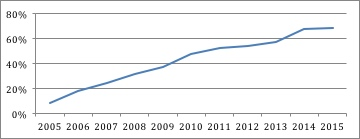
\includegraphics[width=0.5\textwidth]{plots/maxdiffpop}
\end{center}
\end{figure}
MaxDiff, Maximum-Difference Scaling, is a preference measurement and item scaling method.  In a MaxDiff questionnaire the researcher asks respondents for their best and worst item out of a set, then repeats this choice task. Initially proposed by~\cite{louviere1991best}, MaxDiff was first released as a software system in 2004 by Sawtooth Software, a top marketing research software company in North America. Since its release its popularity increased steadily with penetration of the technique, now used by over 70\% of all Sawtooth Software users in 2017 (Figure \ref{fig:pop}). 

MaxDiff offers benefits over alternative methods. MaxDiff provides more discrimination among items and between respondents on the items than traditional rating scales~\cite{cohen2004s}. Besides enhanced discrimination, it avoids the scale use bias so problematic with traditional ratings scales (Louvier; Chrzan).

MaxDiff, while it is a distinct type of choice experiment, is closely related to conjoint. A key difference is that it involves both best and worst choices instead of only one. But in its most common form, MaxDiff may be thought of as a one-attribute CBC study with many levels.  

\subsection{Studying More Items with MaxDiff: Survey of Market Research Practitioners}
MaxDiff has proven so useful that market researchers increasingly find reasons to use MaxDiff for a large number of items.  How many is a large number of items?  In their 2007 paper, Hendrix and Drucker described ``large sets'' as about 40 to 60 items, proposing variants to MaxDiff called Augmented and Tailored MaxDiff to handle such large problems~\cite{hendrix2007alternative}. In their 2012 paper, Wirth and Wolfrath also investigated variants to MaxDiff called Express and Sparse MaxDiff for handling what they described as ``very large sets'' of items~\cite{wirth2012largeset}.  Very large to these authors meant potentially more than 100 items.  To support their findings, they conducted a study among synthetic robotic respondents with 120 items and a real study among humans with 60 items.

For Hendrix and Drucker 40 to 60 items was large, for Wirth and Wolfrath 120 items was very large.  For this current paper, we're referring to huge numbers of items as potentially 300 or more. The motivation of our research is beyond academic curiosity, as marketing researchers are seeking such applications pushing MaxDiff further than it was perhaps ever intended. \\
\begin{figure}
\caption{Sawtooth Customer Feedback Survey 2015. Maximum Number of Items Studied via MaxDiff (top; Mean= 40, Median=30, Maximum=400) and Main Purpose for MaxDiff Study with 41+ Items (bottom) } 
\label{fig:max_and_purpose}
\begin{center} 
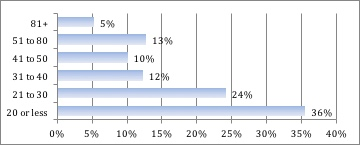
\includegraphics[width=0.7\textwidth]{plots/maxnumstudy}
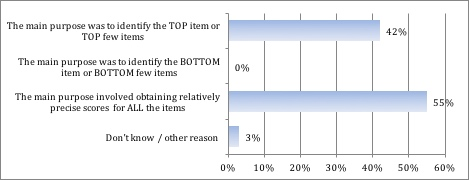
\includegraphics[width=0.7\textwidth]{plots/maxdiffpurpose}
\end{center}
\end{figure}

Sawtooth Software's 2015 Customer Feedback Survey represents users of the software. The survey asked for the largest number of items that users had included in a MaxDiff study during the last 12 months (Figure \ref{fig:max_and_purpose}). Nearly one-fifth of respondents indicated their firms had conducted a study with 51 or more items.  The maximum number of items studied was 400.

To some it may seem odd and overwhelming that some researchers are conducting MaxDiff studies with more than 80 or even 400 items.  However, when we consider that individual MaxDiff items may actually represent conjoined elements that constitute a profile (say, a combination of packaging style, color, claims, and highlighted ingredients), then it can make much more sense to do 400-item studies.  If the profiles involve multiple highly interactive attributes that pose challenges for CBC, then MaxDiff with huge numbers of items could be a viable alternative.

The survey also asked Sawtooth Software customers what the main purpose was for that study with the reported maximum number of items. For studies involving 41 or more items, the main reasons are displayed in Figure \ref{fig:max_and_purpose}. For 42\% of these large MaxDiff studies, the main purpose was to identify the top item or top few items.  

Our research shows that if this is the main goal, then traditional design strategies can be wasteful. We will show that an adaptive approach using bandit algorithms can be about 4x more efficient.  Without the Bandit Adaptive Maxdiff approach, you are potentially wasting 75 cents of every dollar you are spending on MaxDiff data collection. 


%\textbf{Emphasize our goal is to identify the top items.}

\section{Bandit Adaptive MaxDiff}

\subsection{Overview of approach}

Our approach employs an adaptive divide-and-conquer aggregate approach that leverages prior learning to create more efficient questionnaires and more precise aggregate score estimates. We utilize the best available bandit alogrithms and draw upon the active learning and best k arm identification problems.

One efficient solution for solving the multi-armed bandit problem is Thompson Sampling. Thompson Sampling involves allocating resources to an action in proportion to the probability that it is the best action~\cite{thompson1933likelihood}. Any bandit method must find an appropriate balance between exploring to gain information and exploiting that knowledge.

On the one hand, we want to learn about the relative scores of a large number of items within a MaxDiff problem. On the other hand, we want to utilize what we have learned so far to focus our efforts on a targeted set of actions that will likely yield greater precision regarding the items of most interest to the researcher. While there are many methods to accomplish this, Thompson Sampling has proven very useful for these types of problems. For a marketing application of Thompson Sampling and a review of the literature, see \citet{schwartzetal2017}. 

The traditional MaxDiff design approach shows each item an equal number of times across all respondents x tasks.  However, if the main goal is to identify the top few items for the sample, after the first, say 20, respondents it seems reasonable to start paying attention to the already-collected MaxDiff responses and oversampling the items that are already viewed as most preferred (the stars).  We can use aggregate logit to estimate both preference scores and standard errors at any point during data collection (say, after the 20th, 40th, $\ldots$. respondent has completed the survey).

Thompson Sampling makes a new draw from the vector of item preferences using the estimated population preferences (aggregate logit scores) plus normally distributed error, with standard deviations equal to the standard errors of the logit weights.  As the sample size increases, the standard errors of course tighten.
\begin{figure}[!ht]
\caption{Respondent-by-item counts}
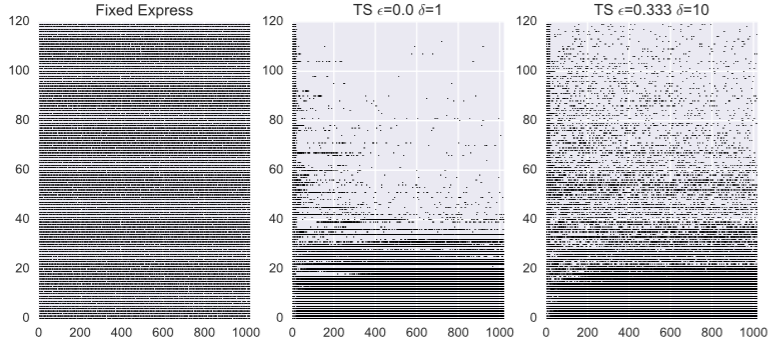
\includegraphics[width=1\textwidth]{plots/3dotplot-lowres.png}
\label{fig:dots}
\end{figure}
To understand the logic of the algorithm, consider a snapshot in time during the data collection. Imagine we have just collected data from 100 respondents, and we decide to summarize their preferences (for each of 100+ items) with aggregate logit.  Then, to generate a MaxDiff task for the 101st respondent, we could generate a draw from the population preferences leveraging the population means and normal errors with standard deviations equal to the empirically estimated standard errors.  We then can sort that newly sampled vector of preference scores from the most to the least preferred item.  The five most preferred items might be taken into the first task to show to the 101st respondent.  The process (with or without updating the logit weights after recording the first task's answer) could be repeated to choose the five items to show in the second task for the 101st respondent, etc.  To reduce the load on the server managing the data collection, perhaps only after every 20th respondent has completed the survey, the logit weights and standard errors would be updated.

We note that the translation of MaxDiff into a bandit problem is not obvious. Our goal is identifying the utilities of the top set of items with maximum precision. Selecting an arm corresponds to including it in the survey for the next respondent. The reward, however, is not as clear. On the one hand, suppose each task included all possible items. Then the reward would be clear: whether the item is chosen as the ``best.'' But it is not feasible to show so many items to respondents, so that's not a relevant scenario. On the other hand, given we only select a subset of items, the item receiving the ``best'' label doesn't translate directly to a reward. Indirectly, that choice data does enable us to infer how it ranks among all items, exactly aligning with our goal. We use the alignment of the managerial goal and the MAB algorithm's balancing of learning and earning to our advantage.


\subsection{Formal Development of Model and Algorithm}

We formalize the proposed procedure in two stages. First, we introduce MaxDiff as a best-worst scaling discrete choice task, and we relate it to the standard multinomial logit model. Next, we introduce adaptive techniques as the natural method for solving the pure exploration problem.

\subsection{MaxDiff choice model}

Every respondent selects both the best and the worst option from an available set of options in each discrete choice task. The model for that data comes from a class of probability models known as best-worst scaling, and MaxDiff is one such model. We adopt the framework from the best-worst scaling literature. For a review, see ~\cite{marley2012models} Marley 2010, ~\cite{marley2005some}. 
We have K possible items, and we select a set S for each choice task. To describe the items, we define two random variables, best $B_z$ and worst $W_z$, for each $z \in S$.  We then define a third random variable, best-worst $BW_{r,s}$, for any $r,s \in S$.\\
Following a random utility framework, these utilities have deterministic and stochastic components.\\ 
A consistent extreme value random utility model is a Thurstone random utility model where each $\varepsilon_z$ has the extreme value distribution. Consistent model means $B_z=-W_z=U_z$ and $BW_{r,s}=U_r-U_s$, then
\begin{align*}
&B_z=v_z+\varepsilon_z\\
&W_z=-v_z-\varepsilon_z\\
&BW_{r,s}=v_r-v_s+\varepsilon_r-\varepsilon_s\\
\end{align*}
We can write the probability that an item is the best and the probability that the item is the worst.
\begin{align*}
&B_S (x)= Pr⁡( B_x=\max_{z \in S} B_z)\\
&W_S (y)= Pr⁡( W_y=\max_{z \in S} W_z)\\
\end{align*}
Without even using the particular utility or scale of items we can derive choice probabilities. In the most general, form we suppose $b()$ and $w()$ are separate interval scales. Then the resulting probability of an item being best or worst is
\begin{align*}
&B_S (x)= \frac{b(x)}{\sum_{z \in S}b(z)}\\
&W_S (y)= \frac{w(y)}{\sum_{z \in S}w(z)}\\
\end{align*}
For any pair of items, $x,y \in S$, we can write the joint probability that $x$ is best and $y$ is worst. However, when considering the best and worst jointly the scales $b$ and $w$ are not separately identified. So we fix their ratio for the same item by setting $w(z)=\frac{c}{b(z)}$. The resulting joint probability is a function of the ratios of scales for pairs of items, 
\begin{align*}
&BW_S(x,y)=Pr(U_x>U_z>U_y | z \in S -\{x,y\}, x\neq y)\\
&BW_S(x,y)=\frac{b(x)/b(y)}{\sum_{r,s \in S, r \neq s}b(r)/b(s)}
\end{align*}
To accommodate the standard utility structure, we let utility $u(z)=\log{(b(z))}$ Then each of the probabilities 
\begin{align*}
&B_S(x)=\frac{e^{u(x)}}{\sum_{z \in S} e^{u(z)}}\\
&W_S(y)=\frac{e^{u(y)}}{\sum_{z \in S} e^{u(z)}}\\
&WB_S(x,y)=\frac{e^{u(x)-u(y)}}{\sum_{r,s \in S, r\neq s} e^{u(r)-u(s)}}
\end{align*}
We can derive the same representation from the random utility model~\cite{marley2005some}. \\
We can view best-worst choice as a generalization of the classic multinomial logit for the choice of the best only.

\subsubsection{Model Estimation}

From our perspective as researchers, all of the utilities are unknown. We can estimate the MaxDiff choice model in a variety of ways. One way to do this exactly is to enumerate all possible pairs of items $x$ and $y$ and then we describe their joint probability of being best and worst, which is the probability of being having the largest difference $BW_S(x,y)$. The pairwise approach scales quadratically in the number of items. We adopt an alternative approach, which reflects the literature and practice and is shown to be a near exact approximation~\cite{cohen2003maximum}. This allows us to estimate the best model and worst model independently, without explicitly estimating the best-worst probability. 
We describe the data for any individual-task combination. Let $Y_{B_S}(z)$ be the binary choice variable, which equals 1 if the item is selected as best in the set $S$, and 0 otherwise. Then $Y_{W_S}(z)$ is the indicator of whether item $z \in S$ is selected as the worst. The design matrix $X_{B_S}$ (of size $|S|$-by-$N$) contains indicator variables taking on value of 1 for each item in the current set $S$ and 0 otherwise. To signal the item as worst, we set $X_{W_S}=-X_{B_S}$, so $X_{W_S}$ contains values of 0 or -1.  Taken together, we express the negative likelihood of the choice data as a multinomial logit with choice probabilities in vector notation as follows,
\[
-\Pi\frac{\exp{(\begin{bmatrix}Y_B\\Y_W\end{bmatrix}\theta)}}{\exp{(\begin{bmatrix}X_B\\X_W\end{bmatrix}\theta)}}
\]
The rows in this matrix representation represent every respondent-task-item combination, $N*J*|S|$, repeated twice.  
The link between the models of best choice and worst choice is the parameter $\theta=\{\theta_1,\ldots,\theta_m \}$. This common parameter vector represents the overall utility of each item $1,\ldots,m$. For a more positive $\theta_i$, the item $i$ has a larger probability of being chosen as best; the more negative, the more likely the item will be chosen as worst.\\
We clarify language about utility, which may diverge from conjoint language or language for multi-attribute profiles. Since $X$ is an indicator, the $\theta$ only represents the utility of item $i$ being included versus excluded. If $\theta_i > \theta_{i'}$, then we say item $i$ is ``more preferred,'' ``more important,'' or simply, ``better.''\\
Due to the sparse nature of MaxDiff for huge numbers of items plus the desire for rapid real time updates, we decided to use aggregate MNL rather than a Bayesian approach.\\
The log-likelihood can be written in summation notation where $S_n$ denotes the nth set of choices as follows
\[
LL(\theta)=-\sum_{n=1}^N \sum_{x \in S_n} (Y_{B_{S_n}}(x)\log{\frac{e^{\theta_x}}{\sum_{z\in S_n} e^{\theta_z}}}+ Y_{W_{S_n}}(x)\log{\frac{e^{-\theta_x}}{\sum_{z\in S_n} e^{-\theta_z}}})
\]
In our work we find $\theta$ by minimizing the negative log-likelihood using Newton-Rapson.

\subsubsection{Characterizing parameter uncercertainty}

For each respondent we select $L$ items, and we generate a MaxDiff design of $J$ best-worst tasks, each with a choice set of $|S|$ items.  We use $L=20$, $J=12$, $|S|=5$ as a default since it is a standard number of items used in MaxDiff studies~\cite{wirth2012largeset}. We begin by selecting the $L$ items uniformly. After an initial number of respondents, we are still uncertain about the each parameter value, so we continue collecting data. But we do not need to reduce that uncertainty equally for each one, so we begin adapting. To translate our current beliefs about parameters into action, we can draw from an exact or approximate posterior distribution and use an adaptive method, explained in detail in the following sections and summarized in table \ref{methods}, to decide what questions to show the next respondent. In the case of the multinomial logit, we can use MCMC to obtain samples, sample from asymptotic distribution via MLE implied by the estimated mean and standard errors, or as we do in the empirical application, use Bayesian bootstrapping. Using Bayesian Bootstrap a draw $u$ is made in the following way.
\begin{align*}
&\beta_1,\beta_2,\ldots,\beta_N \sim \text{exp}(1)\\
&LL(\theta;\beta)=-\sum_{n=1}^N \beta_n\sum_{x \in S_n} (Y_{B_{S_n}}(x)\log{\frac{e^{\theta_x}}{\sum_{z\in S_n} e^{\theta_z}}}+ Y_{W_{S_n}}(x)\log{\frac{e^{-\theta_x}}{\sum_{z\in S_n} e^{-\theta_z}}})\\
&u=\argmin_{\theta} LL(\theta;\beta)
\end{align*}
The adaptive method then use these draws to decide the next $L$ items to show.

\subsubsection{Practical Considerations for Implementation}

There are two practical issue we highlight. First, We want to avoid repeating extremely similar questions to the same respondent. A natural consequence of adaptive methods is convergence: as the sample size grows, certain items achieve high preference scores with smaller standard errors.  Without any additional restrictions, the same few items will eventually tend to be drawn into adjacent MaxDiff tasks for the same respondent, causing much annoyance due to the severe degree of item repetition.  Although this is statistically most efficient, it would drive human respondents mad.  To avoid this, after drawing a fixed number of items (e.g., 20 or 30) to show each respondent,  those draws of 20 items are shown to each respondent in a balanced, near-orthogonal design, leading to a palatable low degree of repetition of items across adjacent sets.  The attentive reader will notice that our approach is quite similar to Wirth's Express MaxDiff approach, except that the logic for selecting the 20 items for each respondent is adaptive leveraging information from the previous respondents-focusing the most recent respondent's efforts on discriminating among items that already have been judged likely to be the stars.

One issue this approach avoids is the respondent tiring out. Instead of trying to create a MaxDiff design with 120 items, which would lead to an unreasonable number of best-worst tasks per respondent, we use the smaller subset of 20.  We also avoid repetition. A particularly annoying alternative is to draw independent samples ranking each choice task for the same respondent. This results in very repetitive choice tasks as parameter estimates.  

The second is frequency of updating the data. If people are taking the survey sequentially then all the data from the previously respondents can be used to generate the surveys for the newcomer. Often this is not the case, as an alternative you can update the data once every $b$ people and decide the questions for the next $b$ people. We call $b$ the batch size and in our empirical analysis we let $b=20$.

Both of these considerations avoid is latency during a survey adn across respondents. Since all the questions for the next $b$ people are set, no computation takes place before or inbetween questions for a respondent. This allows for these methods to be put into practice.

\subsubsection{Base Algorithm: TS}


Taken together, the model's structure, estimation approach with uncertainty, and pracical considerations, we can now describe the base algorithm of Bandit Adaptive MaxDiff with Thompson Sampling (TS). The general approach is seen in Algorithm \ref{alg:general}. The specific instantiation of \ts is seen in Algorithm \ref{alg:ts_simple}


\begin{algorithm}
\caption{General adaptive method} \label{alg:general}
\begin{algorithmic}[1]
\State Initialize 
\State
\State Collect new data from respondents
\State Estimate model parameters
\State Select next questions for respondents
\State Check stopping rule
\end{algorithmic}
\end{algorithm}


\begin{algorithm}
\label{alg:ts_simple}
\caption{Bandit Adaptive MaxDiff: \ts}
\begin{algorithmic}[1]
\State given: $K,L,J,S,b$
\State Initialize first set of questions by sampling $L$ items uniformly
\State Design MaxDiff questionnaire covering $L$ items with $J$ tasks of $S$ questions each, $\text{MDDesign}(L,S,J)$, to the next batch of $b$ respondents.
\State Collect new data from respondents, currently with $n = b*t$ respondents
\State Bayesian Bootstrap sample weight replacement using weights ($\alpha_1, ...., \alpha_n)\sim \text{expon}(1)$ obtaining some subset of $n$ previous respondents.
\State Estimate model parameters. $\theta_t$. Obtain estimated utilities $u = (u_1,...,u_K)$.
\State Choose $L$ items using draws from the empirical posterior
\State Act Select next questions for respondents
\end{algorithmic}
\end{algorithm}

% $S=\#\{\mathcal{S}\}$

With the \ts base algorithm described, we now define reasonable benchmarks from the literature, before moving on to describe the more sophisticated proposed methods. 

\subsubsection{Fixed Express MaxDiff}. We uniformly randomly drew $L$ of $K$ items (without replacement) to show to each respondent.  This achieves balance across items and respondents. For instance, in a problem with $L=20$ of the $K=120$, then each item appears $\frac{J*S}{L} = \frac{12*5}{20} = 3$ times per respondent, on average.

\subsubsection{Algorithm $\epsilon$-greedy}
As a baseline for the adaptive methods will we test the $\epsilon$-greedy. Let $\theta$ be the current estimated parameters. Take the $(1-\epsilon)L$ items with the greatest $\theta$ value and choose the remaining $\epsilon L$ uniformly from the remaining items. For our empirical analysis we use $\epsilon=\frac{1}{4}$ but tested others. Note that greedy alone $\epsilon=0$ would always serve the top $L$ items with the highest estimated average utility to the next respondents.


\begin{table}[ht]
\caption{Summary of Adaptive MaxDiff Algorithms}
\begin{tabular}{p{5cm}|p{11cm}}
Algorithm & Short Description \\
\hline
MaxDiff TS & Sample from the current posterior distribution and serve up the $L$ items with the highest sampled utility.\\
MaxDiff $\epsilon$-Diffuse TS & Sample from the current posterior distribution serve up the $(1-\epsilon)L$ items with the highest sampled utility and sample from the current diffuse posterior distribution and serve up the $\epsilon L$ items with the highest sampled utility not in $(1-\epsilon)L$.\\
$\epsilon$-greedy & Take the $(1-\epsilon)L$ with the greatest current estimated $\theta$. Take the remaining $\epsilon L$ uniformily from the remaining items.\\
TS closest to the threshold & Take the $L$ items that have sampled utility closest to $\frac{u_k+u_{k+1}}{2}$.\\
$\epsilon$-Diffuse TS closest to the threshold & Take the $(1-\epsilon)L$ (from posterior) and  $\epsilon L$ (from diffuse posterior) items that have sampled utility closest to $\frac{u_k+u_{k+1}}{2}$.\\
$\epsilon$-greedy closest to the threshold & Take the $(1-\epsilon)L$ items that have estimated utility closest to $\frac{\theta_k+\theta_{k+1}}{2}$ and $\epsilon L$ items uniformly from the remaining.\\
Misclassification Minimization with random perturbation& Take the $L$ items that have most likely been misclassified (bottom items that should be top items and vice-versa). Add perturbation to the that probability.\\
Greatest Uncertainty with random perturbation& Take the $L$ items whose probabilities of being a top item are closest to 50\%. Add perturbation to the that probability.\\
\end{tabular}
\label{methods}
\end{table}
%%Discuss relation to the Follow the regularized leader / perturbed leader 



\subsubsection{Considerations when implementing Thompson Sampling }

While typical Bayesian or numerical integration methods call for large numbers of draws (or sufficient number) to achieve coverage of the full distribution of parameter values, this  approach relies on the variability of a single sample. There is value in the sample to sample differences in the value of parameters and their relative rank ordering.  

The algorithm learn over time to intuitively achieve the goal of identifying the items with truly high utility with high precision. Early on, we still have substantial uncertainty. The independent samples will differ substantially in rank order of item utilities. This yields MaxDiff designs across respondents with less overlap in items. Later, the uncertainty is reduced most around the truly high-utility items. Across independent samples, the ranking of items will be highly correlated near the top of the ranking (but not near the bottom where uncertainty remains large). As a result, the top subset of $J$ items selected converges to the same group for each respondent. 

One practical issue with Thompson Sampling is robustness to changes overtime. On the one hand, there is built-in robustness. Recall the algorithm is stochastic and adapts continuously. If the early data leads the algorithm astray, then it will self-correct, eventually finding and converging to the truly best items. Suppose the early respondents made choices, by chance, leading us to believe certain items were the best when they were not. The respondents that immediately follow will start receiving these truly poor items. However, as this continues, the uncertainty is reduced around these poor items to reveal there are many other items with probability of being better. By sampling from the joint belief distribution of item utilities, we will be less likely to draw those poor items. One concern is that such sampling could be too aggressive.

\begin{figure}
\caption{MaxDiff TS Illustration}
\label{fig:illustrate_ts}
	\begin{center}
    \subfloat[Early]{{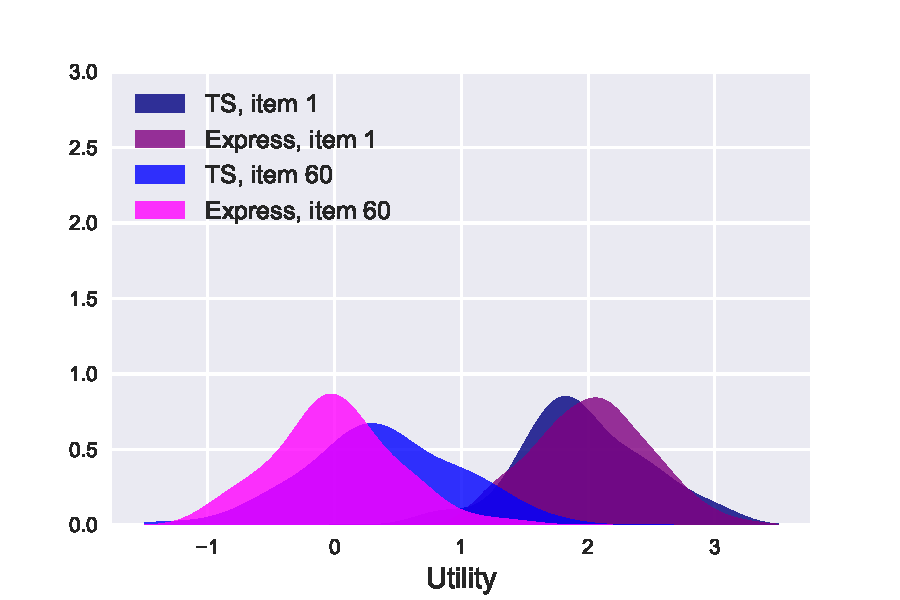
\includegraphics[width=.4\textwidth]{plots/utildis60.pdf} }}%
    \qquad
    \subfloat[Late]{{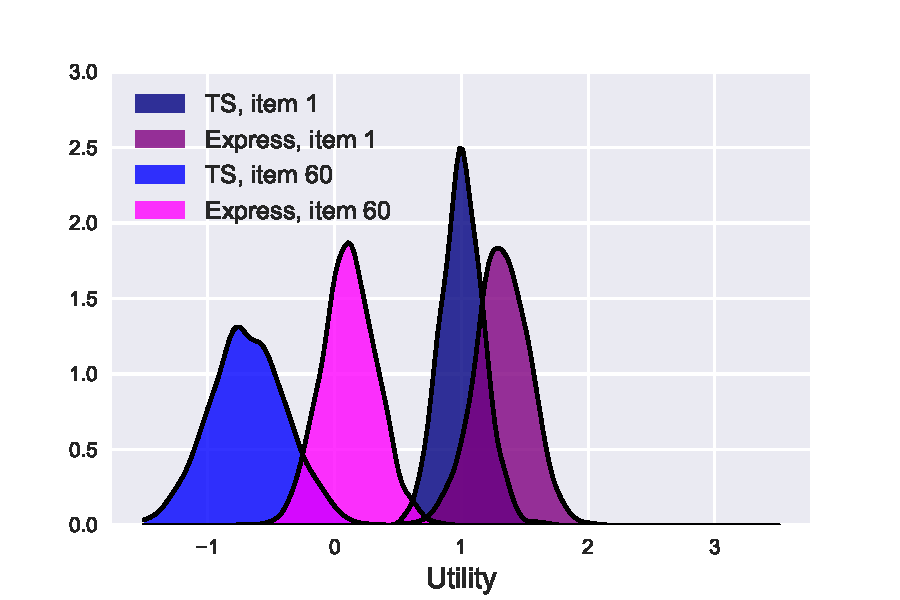
\includegraphics[width=.4\textwidth]{plots/utildis300.pdf} }}%
    \end{center}
\end{figure}



\subsubsection{New Variant of Algorithm: exploration-diffuse ($\epsilon$-$\delta$) TS}
Perhaps the natural parameter uncertainty is not enough or is perhaps too slow to adjust, so we propose an algorithm MaxDiff exploraiton-diffuse TS, or \edts, which has an extra layer of self-correction, making it more robust to non-stationarity or respondent self-selection. The epsilon comes from the popular $\epsilon$-greedy, which mixes greedy with uniform sampling. But instead of being greedy for $1-\epsilon$ samples, this algorithm, follows regular Thompson Sampling. And on $\epsilon$ samples, it does not necessarily sample items uniformly, but it does explore more than regular Thompson Sampling, by drawing parameters a more diffuse posterior distribution, where the variance inflation is controlled by $\delta$.

The \edts is a generalized version of \ts, which directs nests regular \ts. This is analogous to the way a two-component mixture model nests a pooled model without segments. As the $\epsilon \to 0$, the diffuse distribution is never used, so the algorithm collapses to regular \ts. As $\delta \to 1$, the diffuse distribution becomes equivalent to the regular (non-diffuse) distribution. 

To implement \edts, much like any version including Thompson Sampling that we will discuss, the research must choose between approaches for characterizing uncertainty. We contrast Point estimation, using mean and asymptotic variance-covariance, versus using Bayesian Bootstrapping. With the point estimate approach, $\delta$ is directly applied as a variation inflation factor for the estimator (in which case $\delta \geq 1$, with higher values leading to more uncertainty. But with Bayesian Bootstrapping, $\delta$ is the percentage of the data to be used for the bootstrapped sample size, indirectly inflating the estimator's variance. In the Bayesian Bootstrap case, the $0 < \delta \leq 1$, with lower values leading to more uncertainty in the estimate across bootsrapped samples.

The \edts version intuitively hedges its bets on the best items .  As in illustration, instead of sampling 20 items all from \ts, we only sample 15 of 20 items using standard \ts (hence, $L=20$, $\epsilon=1/4$), and the remaining 5 of 20 items are drawn using \ts with a much more diffuse prior (subsampling $\delta$=.25 of the data with replacement and drawing $u$ as a Bayes bootstrap of the subsampled data). Figure \ref{fig:illustrating_edts} illustrates how \edts differs from \ts. 

\begin{figure}
\caption{ Illustration of \ts vs \edts for two items (1st top; 60th, bottom) at two points in time (left, early; right, late). This shows the \ts, \edts belief distributions, and the underlying diffuse distribution in \edts. We show this for early beliefs after respondent 40 (left column of plots) and late beliefs after respondent 500 (right) show learning. }
\label{fig:illustrating_edts}
 	\begin{center}
    \subfloat[Early, 1st rank]{{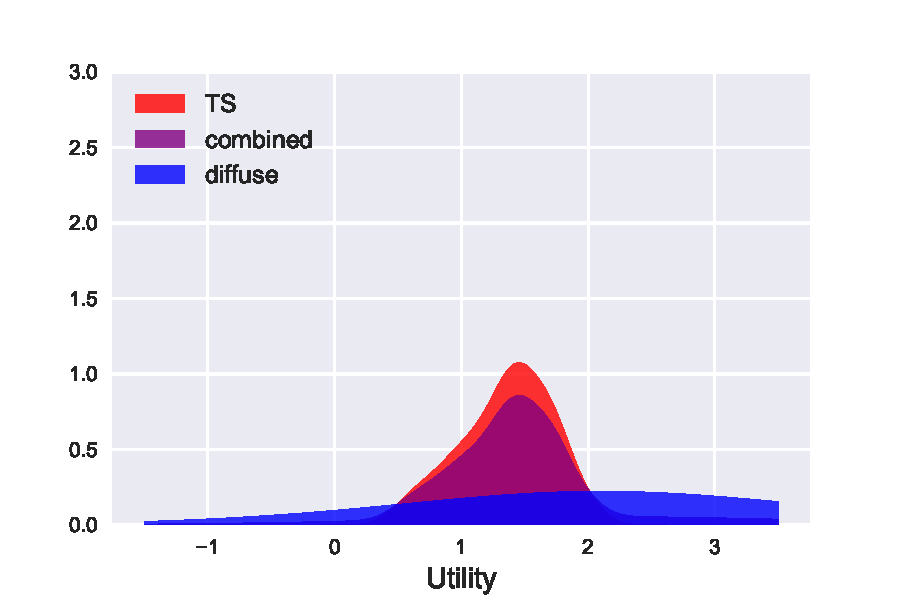
\includegraphics[width=.4\textwidth]{plots/utildifdis600.pdf} }}%
    \qquad
    \subfloat[Late, 1st rank]{{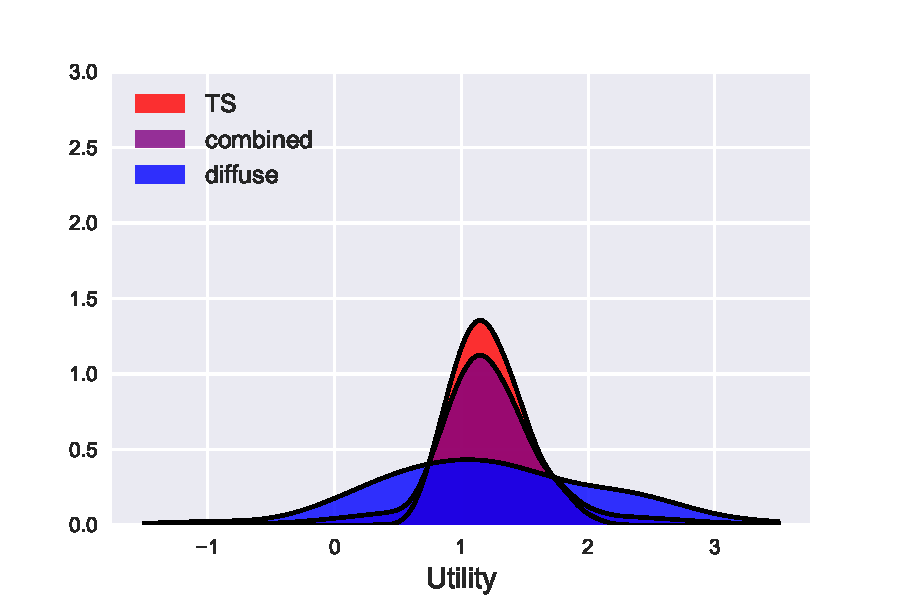
\includegraphics[width=.4\textwidth]{plots/utildifdis3000.pdf} }}%
    \qquad
    \subfloat[Early, 60th rank]{{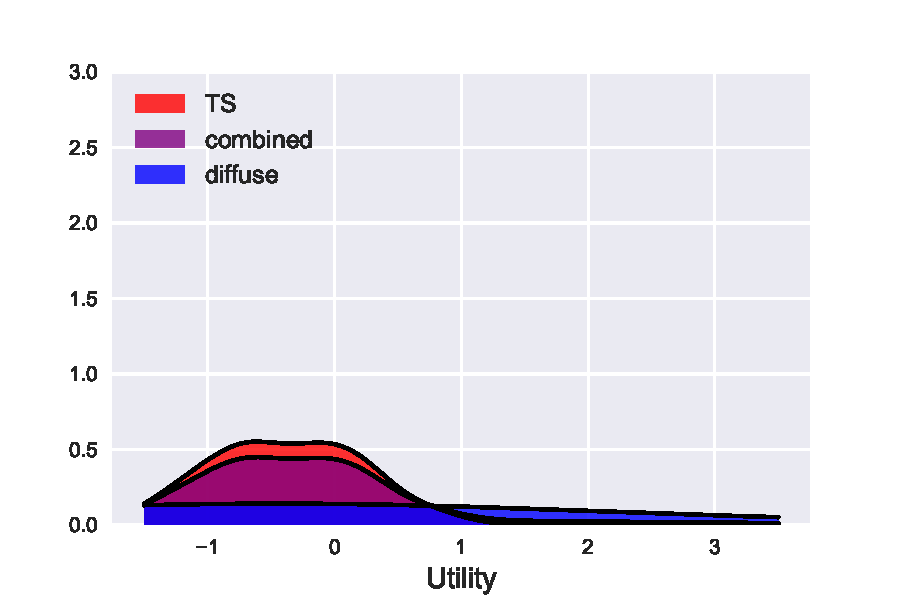
\includegraphics[width=.4\textwidth]{plots/utildifdis6060.pdf} }}%
    \qquad
    \subfloat[Late, 60th rank]{{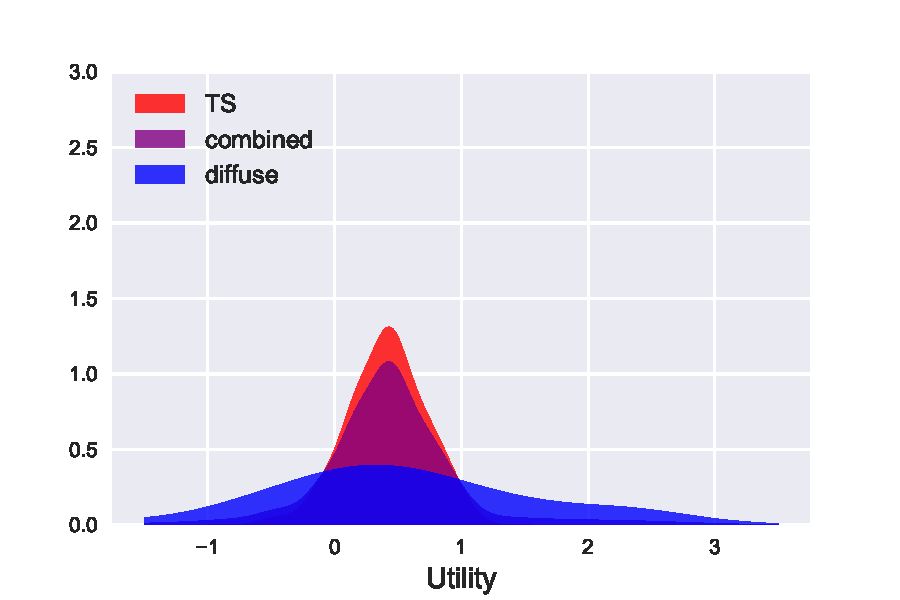
\includegraphics[width=.4\textwidth]{plots/utildifdis30060.pdf} }}%
    \end{center}
\end{figure}


For $\epsilon$-$\delta$ case, its density does not become a spike as quickly as it does without $\epsilon$-$\delta$ . This speed is controlled through two parameters: epsilon, the proportion of items sampled from the diffuse distribution, and $\delta$, factor increasing variance for the diffuse distribution.  The larger the $\epsilon$ and the smaller the $\delta$, the more exploration and slower the algorithm settles on its set of items. 

% \begin{figure}[!ht]
% \caption{Selecting your $\epsilon$-$\delta$ values. 
% 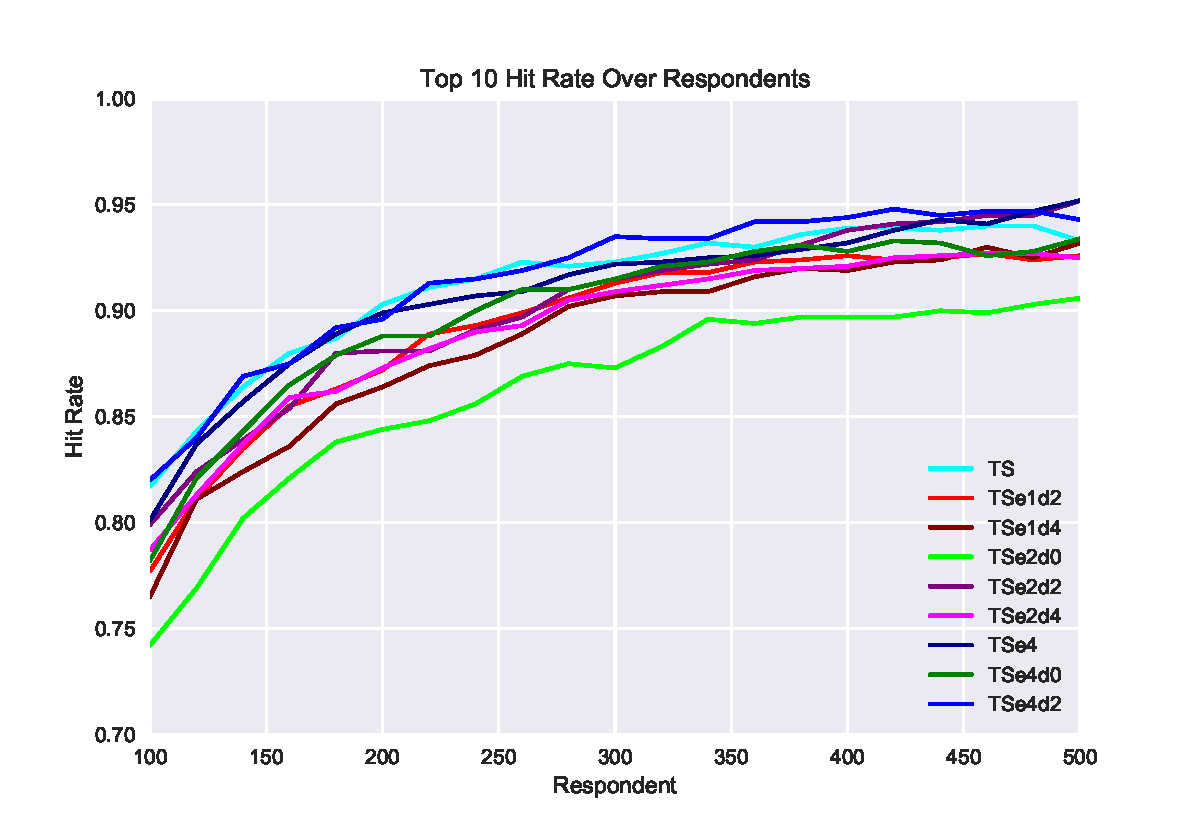
\includegraphics[width=1\textwidth]{plots/hr120v20k10ed.pdf}
% \label{fig:ed}
% \end{figure}

We show how \edts performance varies with different values of $\epsilon$ and $\delta$ in Section \ref{sec:empirical_main}.  For our empirical analysis, we use ($\epsilon=\frac{1}{4}$, $\delta=\frac{1}{4}$). Also tested were ($\epsilon=\frac{1}{2}$, $\delta=\frac{1}{4}$) and ($\epsilon=1$, $\delta=\frac{1}{4}$) which performed on par with ($\epsilon=\frac{1}{4}$, $\delta=\frac{1}{4}$). Our recommended ranges for the parameters are $\frac{1}{5}\leq \epsilon \leq \frac{1}{2}$, $\frac{1}{4}\leq \delta \leq \frac{1}{2}$.\\

%\eric{ AZ will re-run tests on \edts for different combinations of values of $\epsilon=1/2,1/4,0$ and $\delta=1,1/2,1/4,nearly 0 effectively uniform)$, almost do the whole crossproduct except avoid redundancies.} \alexander{to ES: Which ones do you want to keep? see figure \ref{fig:ed}} 




\subsubsection{New Variant: Closest to the Threshold}

In~\cite{toubia2007adaptive}, they introduce Closest to Threshold based on Bradlow and Wainer’s (1998) recommendation
``select ideas near the cutoff''. We also will do that to find the top $k$. For a draw $u$ calculate the cutoff $c=\frac{u_k+u_{k+1}}{2}$ a score $s_i=|c-u^i|$ for every item. Then take the $L$ items with the lowest score. Similarly, we can define $\epsilon$ diffuse version here. For two draws $u_R$ (posterior) and $u^D$ (diffuse posterior) and calculate scores $s_R$ and $s_D$. Take $(1- \epsilon)L$ items with lowest $s_R$scores and the $\epsilon L$ items with the lowest $s_D$ scores not already included. We will also test the $\epsilon$ - greedy version where the scores are $s_i=|c-\theta^i|$ for $c=\frac{\theta_k+\theta_{k+1}}{2}$ you take the $((1-\epsilon)L)$ lowest scores and the rest uniformly.

\begin{verbatim}
       utilities        rank ordering
item : a b c d e f   max(1)(2)(3)(4)(5)(6)min
draw1: 6 7 7 8 8 9  -->  f  d  e  c  b  a   
draw2: 7 5 5 9 8 6  -->  d  e  a  f  b  c 
draw3: 6 4 5 8 7 5  -->  d  e  a  c  f  b 
\end{verbatim}

\subsubsection{Algorithm Misclassification Minimization}
Adapted from~\cite{toubia2007adaptive}, define the score, $s_i$ for each item as follows. If the $i$th item is estimated to be a bottom item the score is $s_i=\mathbb{P}(\text{item i is in the top k})$. If the $i$th  item is estimated to be in the top $k$ then the score is $s_i=\mathbb{P}(\text{item i is not in the top k})$. You can estimate this quantity by taking a large number of draws from the posterior distribution. You take the $L$ items with the highest score.

\subsubsection{Algorithm Greatest Uncertainty}
You define the score, $s_i$ for each item as follows. $s_i=|.5-\mathbb{P}(\text{item i is in the top k})|$. You can estimate this quantity by taking a large number of draws from the posterior distribution. You take the $L$ items with the lowest score.

\subsubsection{Variant Random Perturbation}
From~\cite{toubia2007adaptive}, after calculating the scores for a respondent, you perturb the scores by a normal vector with mean zero and variance $c\frac{1}{n_i}$, Where $n_i$ is the number of questions that has had item $i$ and $c$ is some constant, we take it to be $\frac{1}{10}$ (also tested ws $c=\frac{1}{2}$ which preformed similar). Using the pertubed scores Serve up the $L$ items accordingly. Our recommended range for the parameter is $.01 \leq c \leq 1$\\
The reason for using a variance that decreases over time rather than a fixed variance can be found in ~\cite{toubia2007adaptive} where the author derived insight from genetic algorithms. This method avoids misclassifying an item that will not be sampled further.\\
Additionally if you are using a batch size greater than one, Misclassification Minimization and Greatest Uncertainty would show the same items to all of the respondents. After getting scores that are the same for the next $b$ respondents adding the perturbation vector adds variety to the items shown. This is useful because using Bayes bootstrapping for estimating probabilities required in Misclassification Minimization and Greatest Uncertainty takes a good deal of time since you are optimizing the negative log-likelihood a large number of times.

%=========================
%%%%%%%%%% [ERIC'S EDITING ENDS HERE FOR NOW 2018-01-31] 
%=========================




\section{Empirical Analysis: Main Results}

\label{sec:empirical_main}
We compared our proposed set of adaptive approaches to existing adaptive and non-adaptive strategies. We use simulated choice data based on inferred preferences from an actual MaxDiff survey.

\subsection{Data}
The data come from from a survey conducted by a Procter \& Gamble with Sawtooth Software. The study involved 981 respondents and 120 items. The subject matter and exact item text was hidden for confidentiality purposes. As is common in MaxDiff surveys, the items represented product features and benefits. The questions were came from a sparse MaxDiff study, so this was a fixed non-adaptive design, with balance across all items and respondents. 

Instead of raw choice data, they provided us with the individual-level posterior mean utilities for all respondents and items, which were obtained via Markov Chain Monte Carlo sampling for a hierarchical Bayes (HB) logit model. We call those individual-level utilities the true HB utilities.  These HB utilities offered realistic patterns of preferences across the items and respondents and became our data-generating process for use in our respondent simulations.  Therefore Our simulated respondents mimicked the actual respondents' preferences, on average: to answer each new MaxDiff task, we perturbed those true HB utilities by iid Gumbel distributed error.  

\subsection{Simulation Setup}
To measure performance, we consider a range of metrics: the estimated rank order of items' utilities, the hit rate of whether the estimated top-ranked set of items is correct, the value of the utilities of that estimated top set, and the variability around the estimated utilities. We obtain these measures by comparing estimates to true values. For each batch of respondents, we ran aggregate logit and compare the current rank order of the estimated utilities to the true rank order for the known true utilities, which are the aggregate average across all respondents' true individual-level utilities. We ran the simulations 100 independent runs to obtain a distribution of measures. 

Since we motivated the problem with identifying a top set of items, our primary performance measure is \textbf{top $k$ hit rate}.\textbf{Top $k$ hit rate}: What percent of the true top $k$ items appear in the estimated top $k$ set? For instance, for the top-10 hit rate, if the estimated scores identified 7 of the true top 10 items, irrespective of order, the hit rate was 70\%. We use $k=3,10,20,40$. 

Hit rate is a natural consideration in an active learning problem. It evaluates the quality of the adaptive learning procedures with respect to the eventual decision. Hit rate is also related to regret in a typical multi-armed bandit problem. It reflects how far we are from always selecting the truly best set of arms for all time periods. Again, this is only related but not equivalent to a bandit setting, since it is not exactly an observed reward in the sense of the usual bandit setting (e.g., clicks, purchases). 

\begin{figure}[!ht]
\caption{True utilities of each item learn. The plot shows the rank ordering and values of the utilities on the logit scale for all 120 items, highlighting the top 10 (blue) and top 3 (red). These are the means for unobserved data-generating process.}
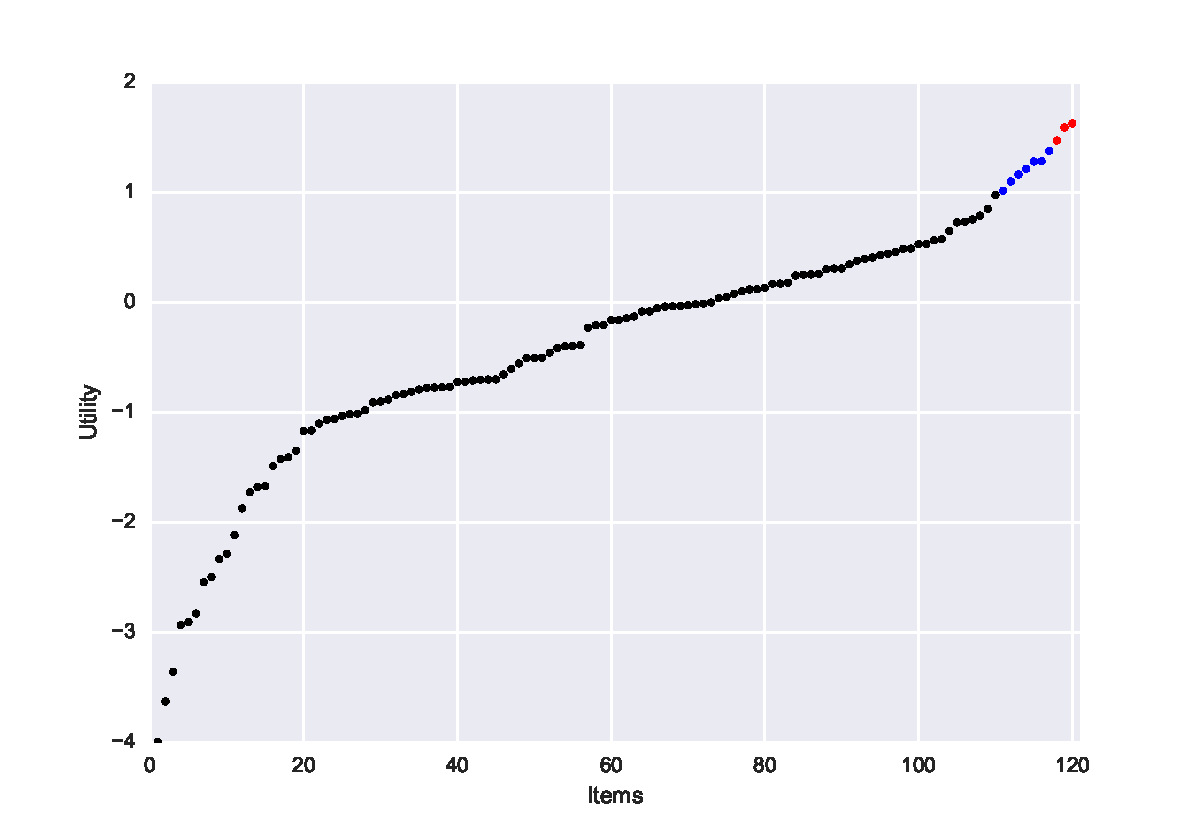
\includegraphics[width=1\textwidth]{plots/utilscore.pdf}
\label{fig:util} 
\end{figure}

The difficulty of identifying the truly best items is related to the differences among those top item utilities (Figure \ref{fig:util}). With 120 items in the dataset, we observed the true preferences for the approximately the top 15 were close in terms of utility (within 1.0 on logit scale). There were no runaway winners. Due to how tightly the top items are clustered, the hit rate measures we employed were quite discriminating between competing methods.

We describe the \emph{base setting}. We simulate the process of collecting survey data from $N=500$ respondents, in batches of $b=20$ respondents per period, using bootstrap sampling, with replacement from the original 981 individuals. We consider the first 20 respondents to be the initial group, which always received $L=20$ items uniformly selected for all methods. All adaptive methods only begin after the 20th respondent. Each simulated respondent completed $J=12$ choice sets (best-worst tasks), where each set included $S=5$ items.

As described earlier, we tested the different adaptive approaches found in Table \ref{methods}. For our base settings, we use ($\epsilon=\frac{1}{4}$, $\delta=\frac{1}{4}$) for $\epsilon-\delta$TS methods. The natural benchmark is the existing fixed MaxDiff approach.


\subsection{Results: Greedy, Thompson Sampling (TS), $\epsilon-\delta$ TS vs Fixed Express}

The first result shows adaptive methods, even simple ones, are better than static ones. But a simple greedy algorithm, which adapts, but does not explicitly incorporate learning, is not good enough. Table \ref{fig:simple_result} shows how TS improves substantially over greedy, and $\epsilon-\delta$ TS adds even more improvement in hit rate.

\begin{figure}
\caption{Adaptive vs Static. Performance is cumulative hit rate per number of respondents so far. The plots show \fixedexpress, \egreedy, \ts, and \edts for k=3, K=120, L=20.}
\label{fig:simple_result}
\begin{center}
	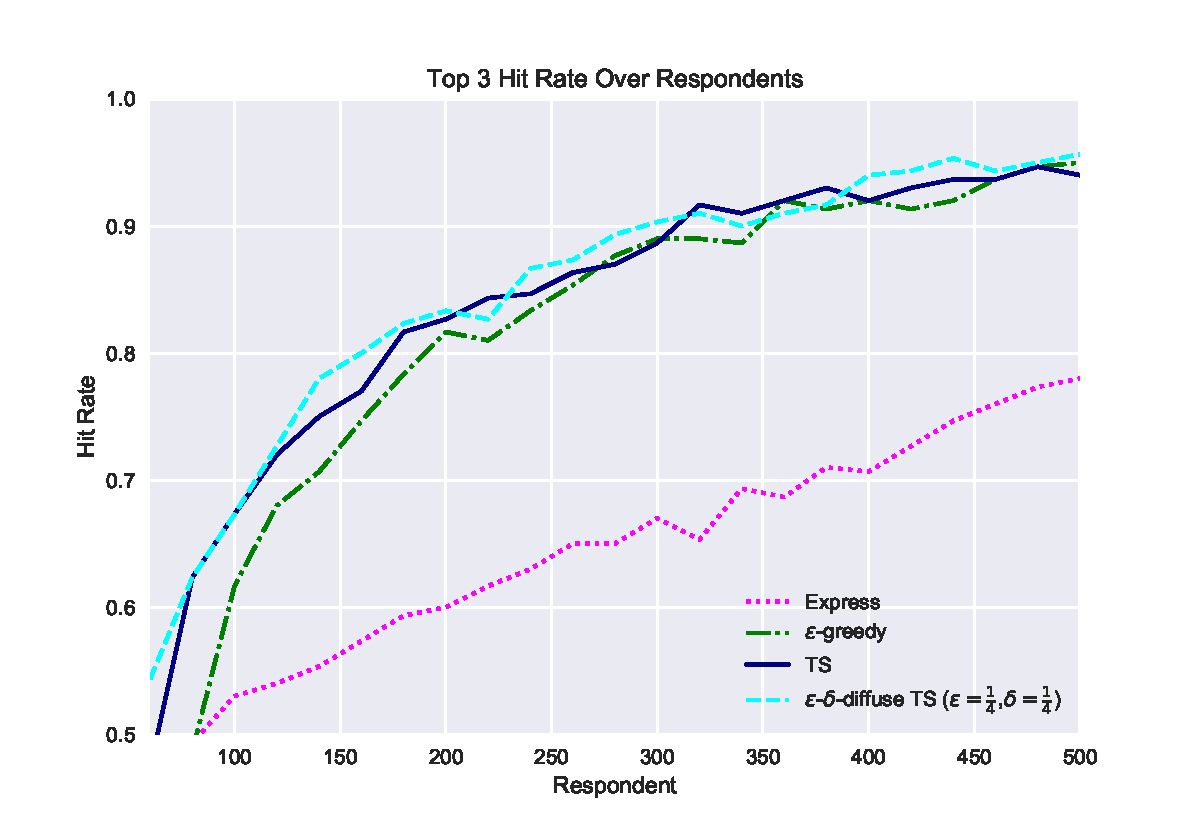
\includegraphics[width=.8\textwidth]{plots/hr120v20k3.pdf}
\end{center}
\end{figure}

For example, after the first 200 respondents, the Fixed Express Design obtains a top 3 hit rate of 60\% whereas the TS-based approaches achieve a top 3 hit rate of about 80\%. Practically, if a marketing researcher wants a hit rate of 80\%, for example, then these methods can achieve that with a smaller sample size. A good adaptive method is at least \emph{three times more efficient} than the standard Fixed Express MaxDiff approach. This holds for the different values tested in the basic setting. 

Figure \ref{fig:effects_epsilon_delta} shows the way the $\epsilon$ and $\delta$ affect the performance. 

\begin{figure}
\caption{How \edts varies with $\epsilon$ and $\delta$. The plots show $\epsilon = 1/2$ (left) and $\epsilon = 1/4$ (right), with multiple lines in each plot, $\delta = 1/2$ (one color) and $\delta = 1/4$ (another color). And in each of the plots also show regular \ts ($\epsilon = 0$,$\delta =1$)}.

\label{fig:effects_epsilon_delta}
 	\begin{center}
    \subfloat[$\epsilon=1/2$]{{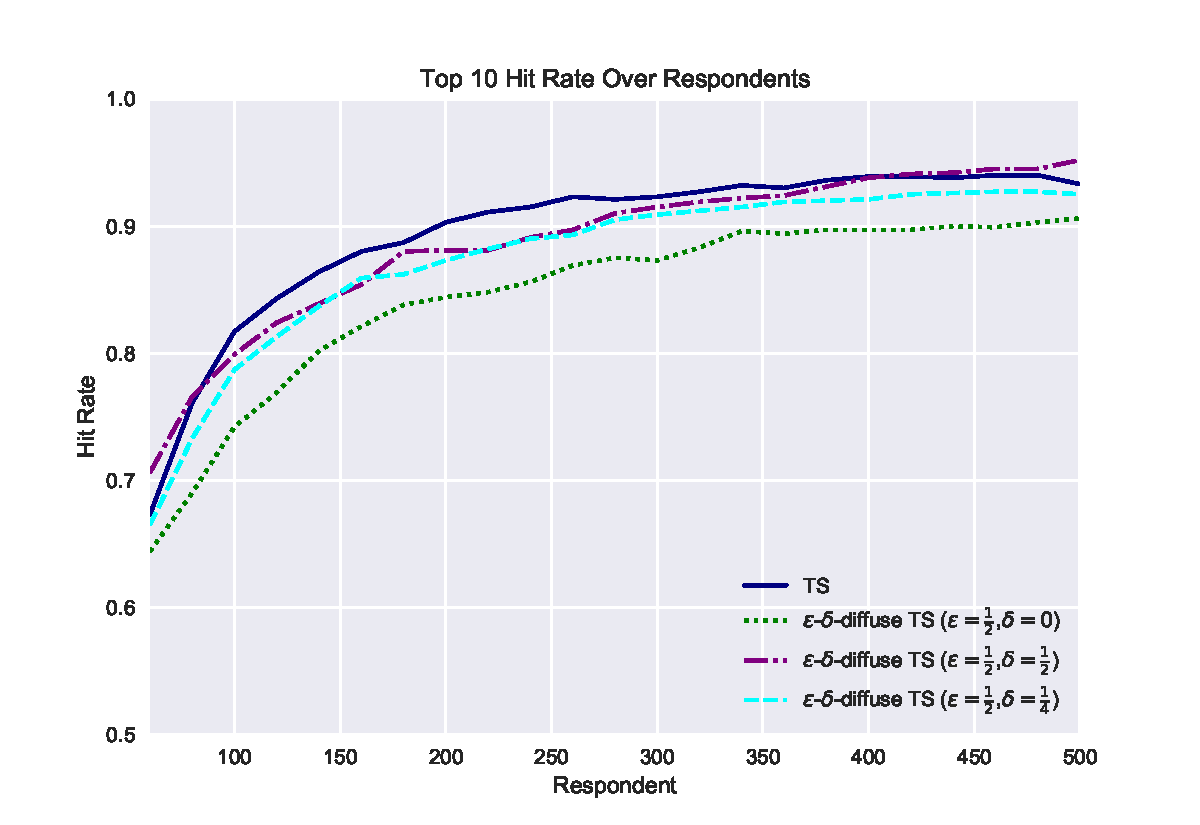
\includegraphics[width=.4\textwidth]{plots/hr120v20k10e2.pdf} }}%
    \qquad
    \subfloat[$\epsilon=1/4$]{{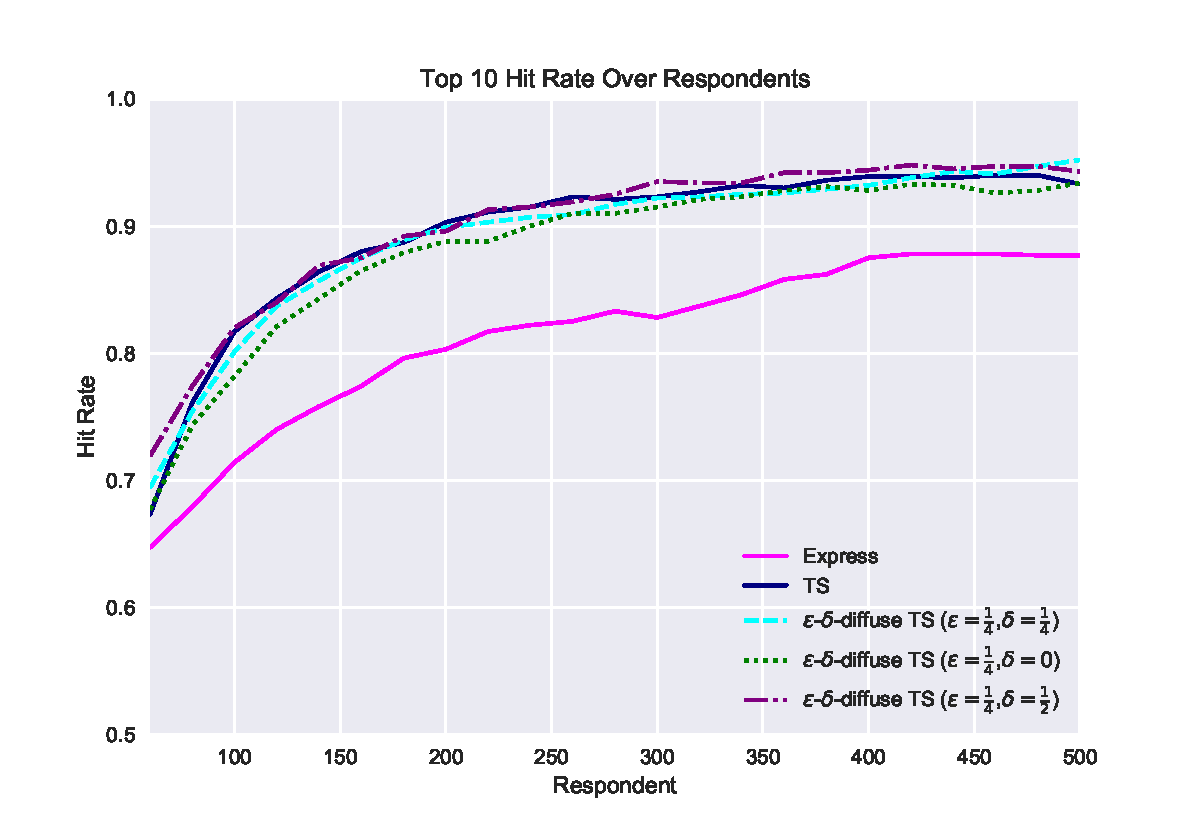
\includegraphics[width=.4\textwidth]{plots/hr120v20k10e4.pdf} }}%
    \end{center}
\end{figure}


We will later show the performance gap between \ts and \edts widens dramatically when considering non-stationary settings, such as with a misinformed starts in Section \ref{sec:robust}. 


\subsection{Results: Thresholding, Uncertainty reduction (\uncert), Misclassification (\mismin) }

However, we next examine the other proposed methods. Recall each algorithm selects $L=20$ items to serve to every respondent. But we examine hit rate for the top $k$ items, for $k = \{3,10,20,40\}$. Overall, a smaller $k$ makes the problem more challenging to do well earlier, since a hit rate for the top 3 out of 120 is a higher bar than the hit rate for 40 out of 120, especially in light of the distribution of true utility values (Figure \ref{fig:util}).  


Figures \ref{fig:K120_L20_k3hit_k10hit} and \ref{fig:K120_L20_k3hit_k10hit} and Table \ref{table:at_260_500} show the results for the $K=120$-item dataset serving $L=20$ questions per respondent, where all methods were tested.


\begin{figure}%
    \caption{Effects of Thresholds for Hit Rates for Top $k=\{10,20\}$ with 120 items. The cumulative hit rate obtained (y-axis) improves with the number of respondents interviewed (x-axis), but it does so at different rates for each algorithm.}%
    \label{fig:K120_L20_k3hit_k10hit}%
 	\begin{center}
    \subfloat[Top 10]{{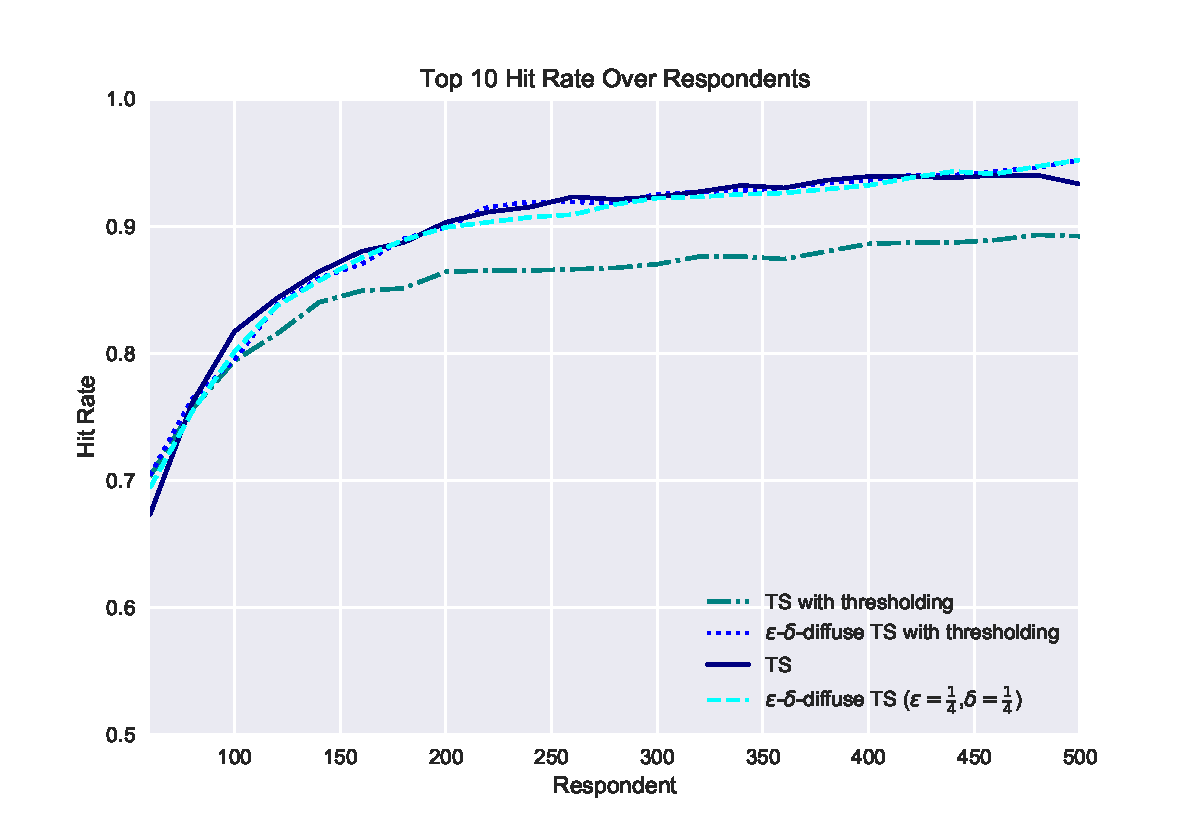
\includegraphics[width=.8\textwidth]{plots/hr120v20k10thres.pdf} }}%
    \qquad
    \subfloat[Top 20]{{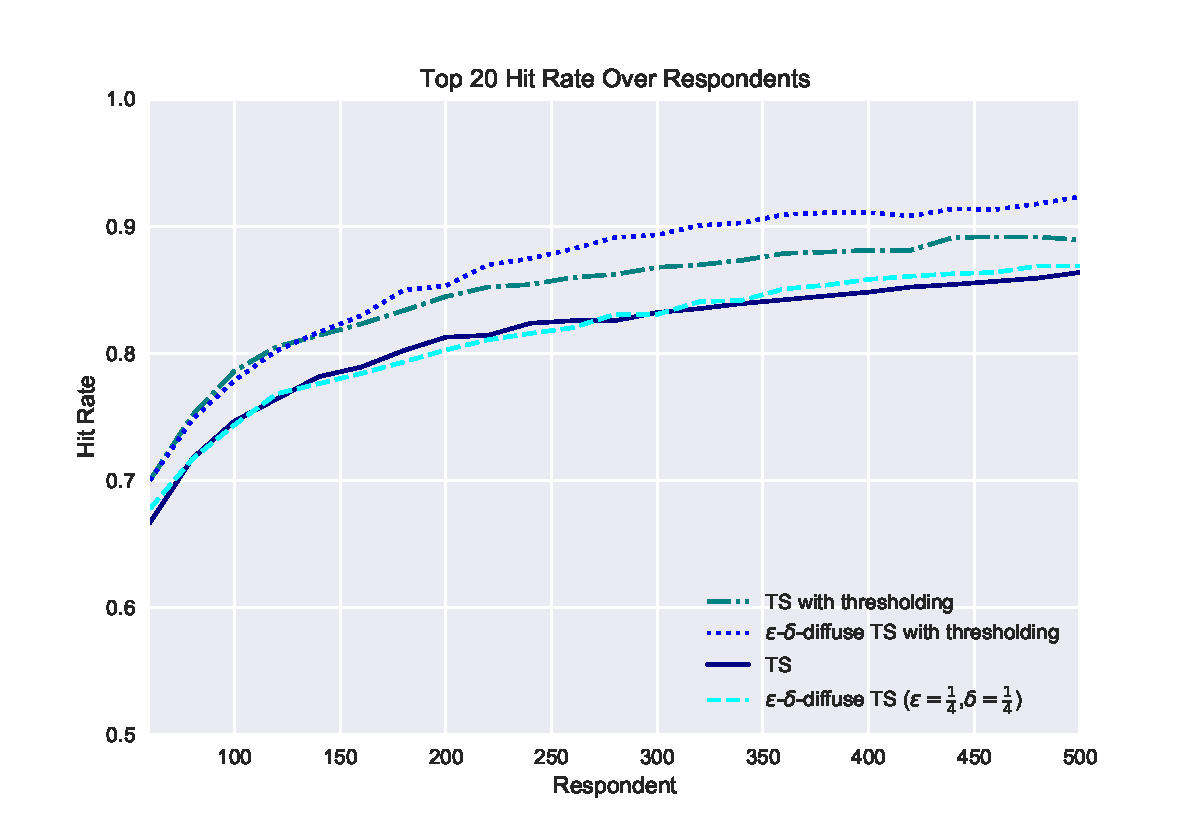
\includegraphics[width=.8\textwidth]{plots/hr120v20k20thres.pdf} }}%
	\end{center}
\end{figure}
%\eric{Please make y-axes the same across all k for the K120 L20 problem. Only show \fixedexpress,\egreedy, \ts,\edts with usual values, and their thresholding counter parts, \egreedythres, \tsthres, \edtsthres. Why is \ts better than \tsthres for $k=10$?  Explain why in a good way \tsthres always does worse than \edtsthres. }

\begin{figure}%
    \caption{Hit Rates for Top $k=20$ with 120 items, 20 items per person. The cumulative hit rate obtained (y-axis) improves with the number of respondents interviewed (x-axis), but it does so at different rates for each algorithm. }%
    \label{fig:K120_L20_k3hit_k10hit}%
 	\begin{center}
    \subfloat[Top 20]{{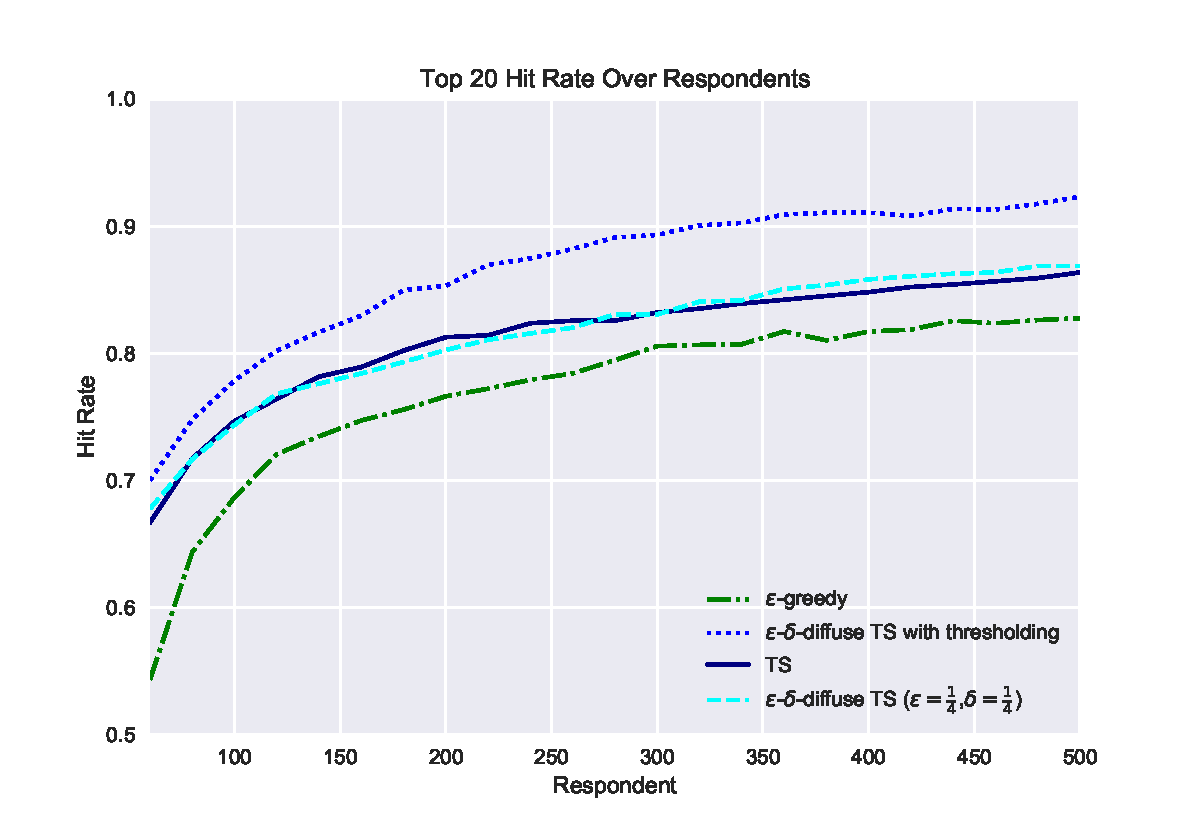
\includegraphics[width=.8\textwidth]{plots/hr120v20k20t.pdf} }}%
    \qquad
    \subfloat[Top 20]{{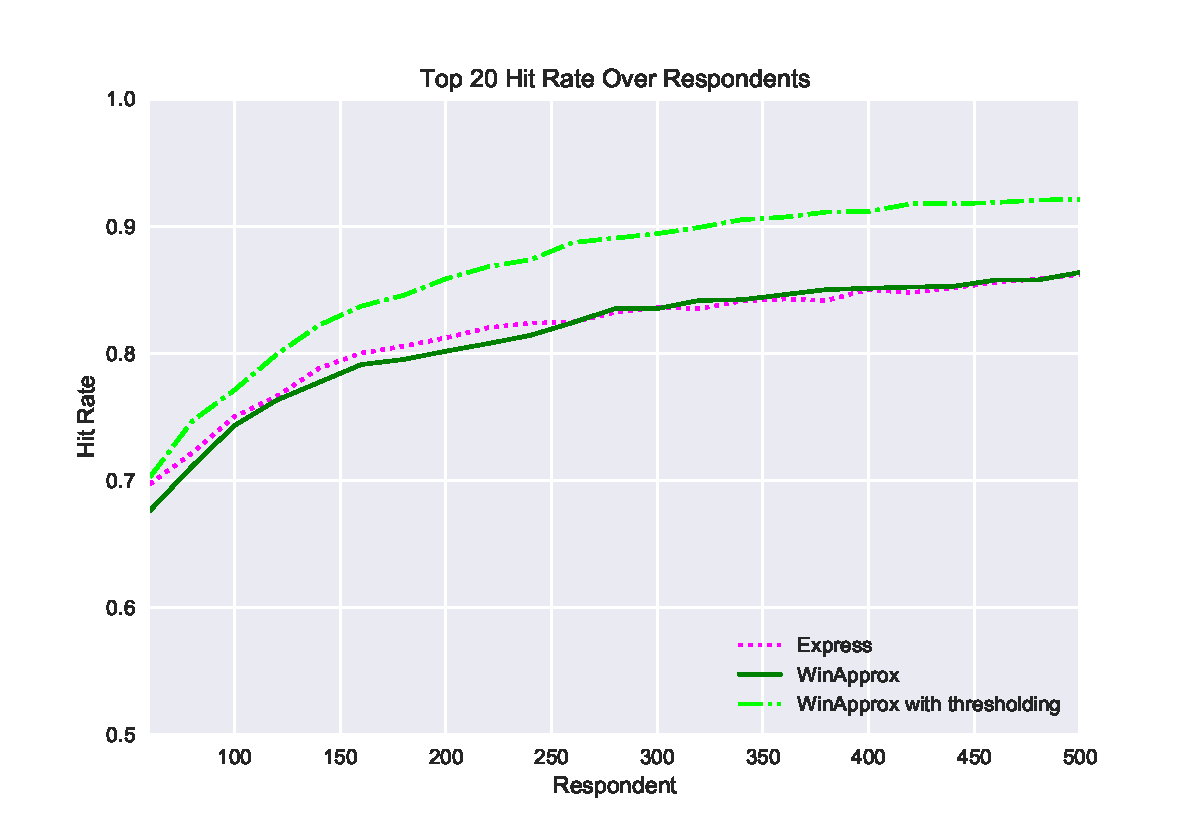
\includegraphics[width=.8\textwidth]{plots/hr120v20k20t2.pdf} }}%
	\end{center}
\end{figure}

%\eric{\fixedexpress, \egreedy, WinApprox (for later), \ts,\edts with usual values, \edtsthres.}


\begin{figure}%
    \caption{Hit Rates for Top $k=\{3,10\}$ with 120 items. The cumulative hit rate obtained (y-axis) improves with the number of respondents interviewed (x-axis), but it does so at different rates for each algorithm.}%
    \label{fig:K120_L20_k3hit_k10hit}%
 	\begin{center}
    \subfloat[Top 3]{{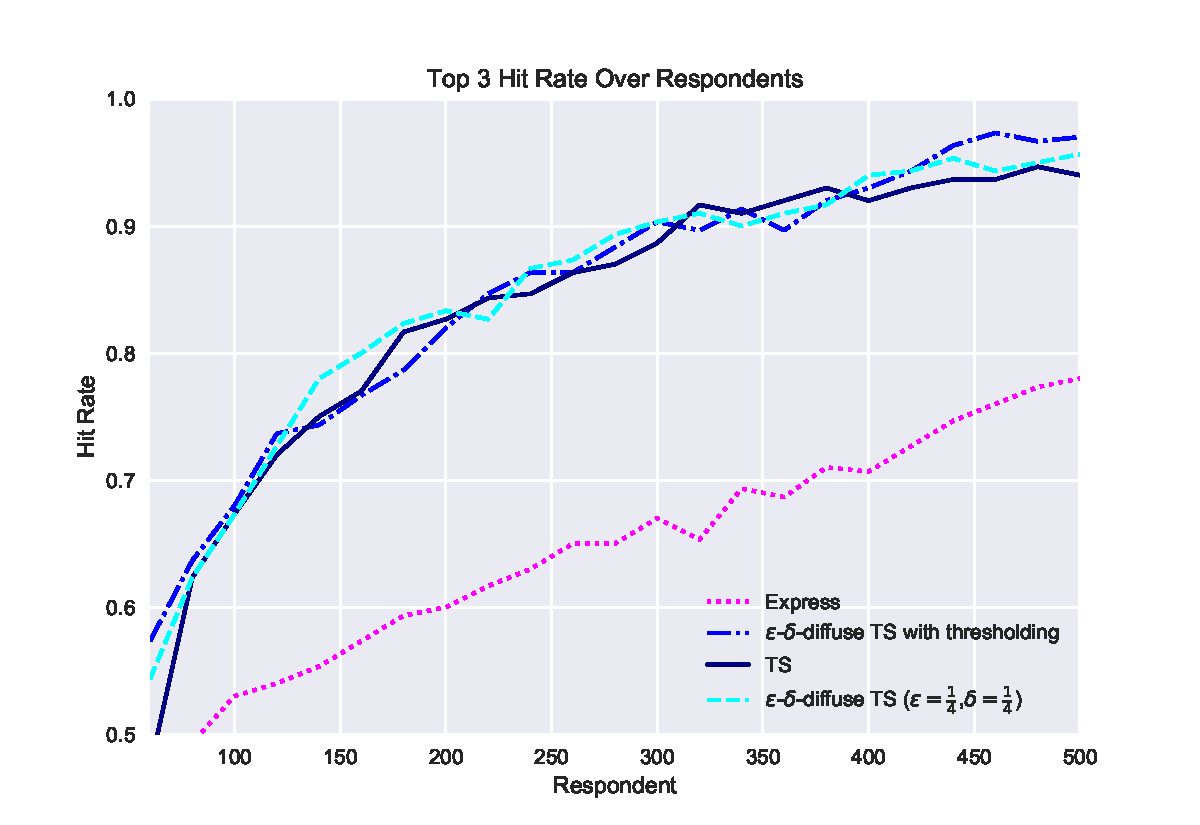
\includegraphics[width=.8\textwidth]{plots/hr120v20k3TS.pdf} }}%
    \qquad
    \subfloat[Top 10]{{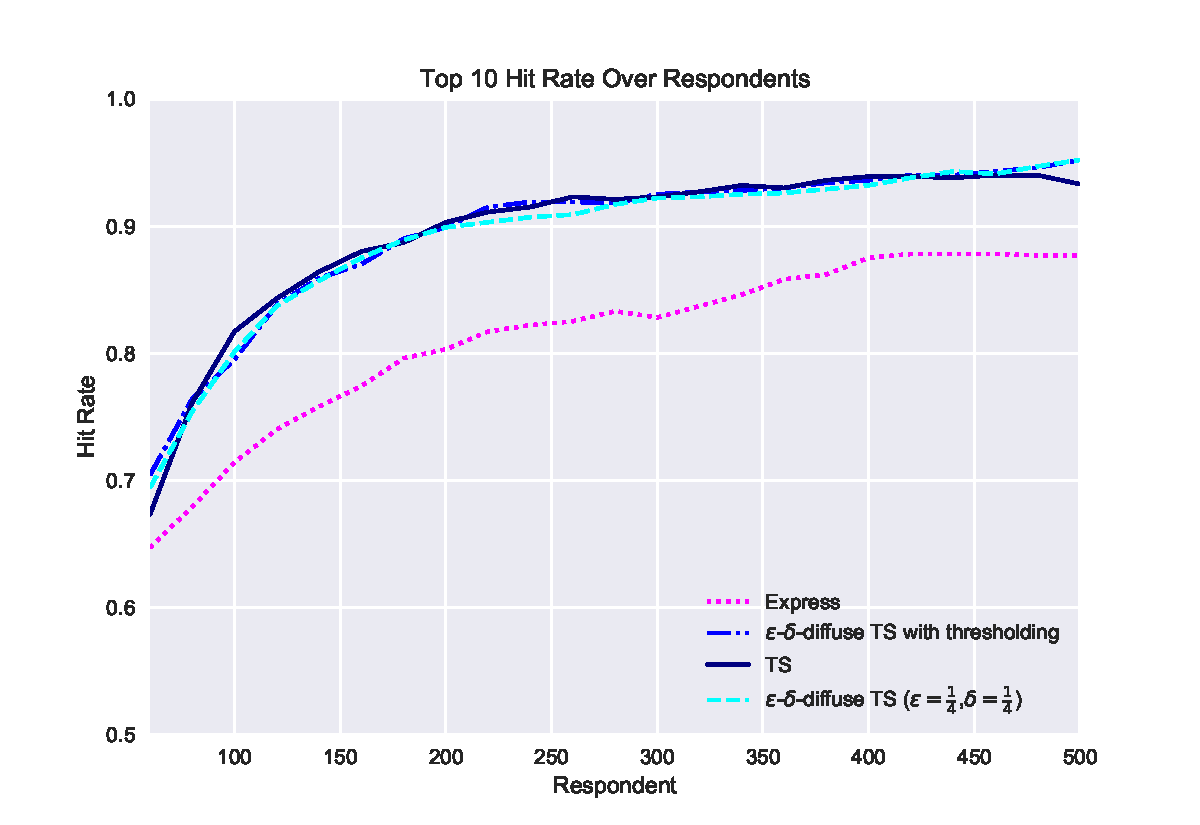
\includegraphics[width=.8\textwidth]{plots/hr120v20k10TS.pdf} }}%
	\end{center}
\end{figure}

 %\eric{Please make y-axes the same across all k for the K120 L20 problem. Only show \fixedexpress, \ts,\edts with usual values, \tsthres, \edtsthres. Why is \ts better than \tsthres for $k=10$?   }

\begin{figure}%
    \caption{Hit Rates for Top $k=\{3,10\}$ with 120 items. The cumulative hit rate obtained (y-axis) improves with the number of respondents interviewed (x-axis), but it does so at different rates for each algorithm. The plots show \fixedexpress, \edtsthres, \mismin, \uncert }%
    \label{fig:K120_L20_k3hit_k10hit}%
 	\begin{center}
    \subfloat[Top 3]{{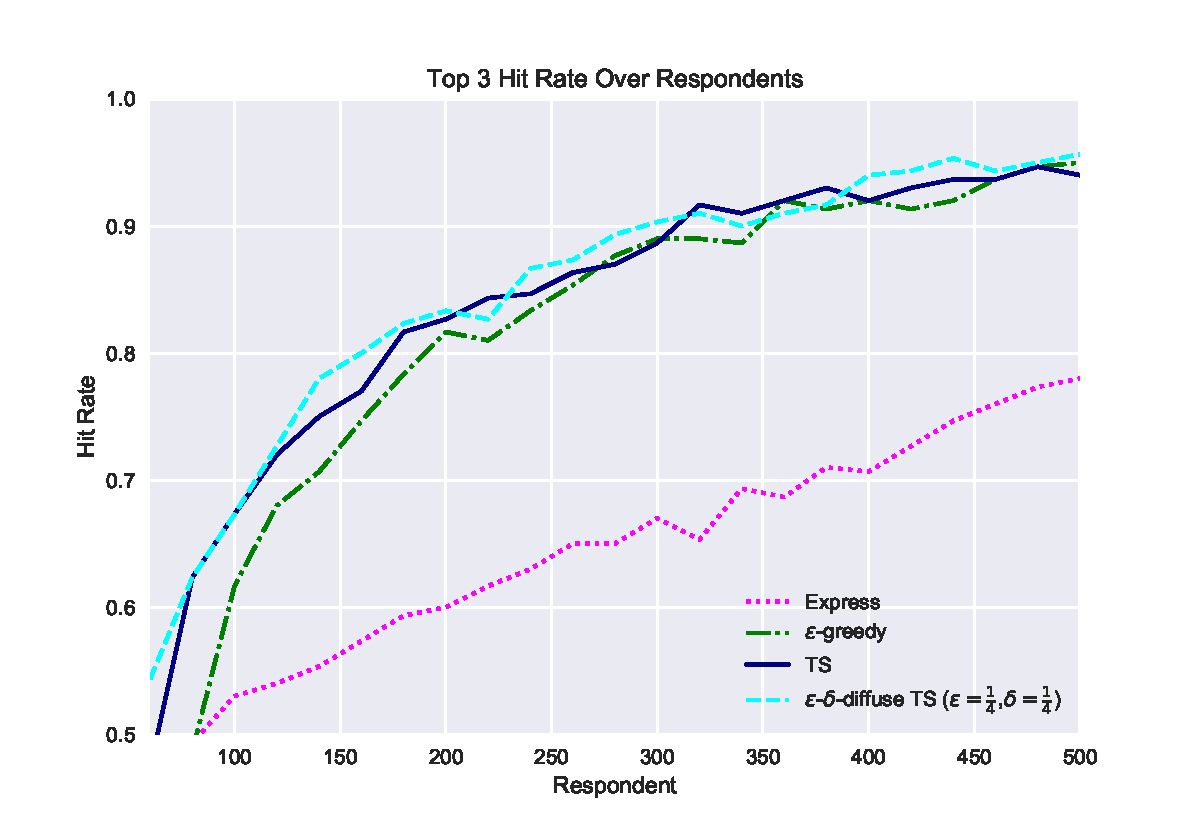
\includegraphics[width=.8\textwidth]{plots/hr120v20k3.pdf} }}%
    \qquad
    \subfloat[Top 10]{{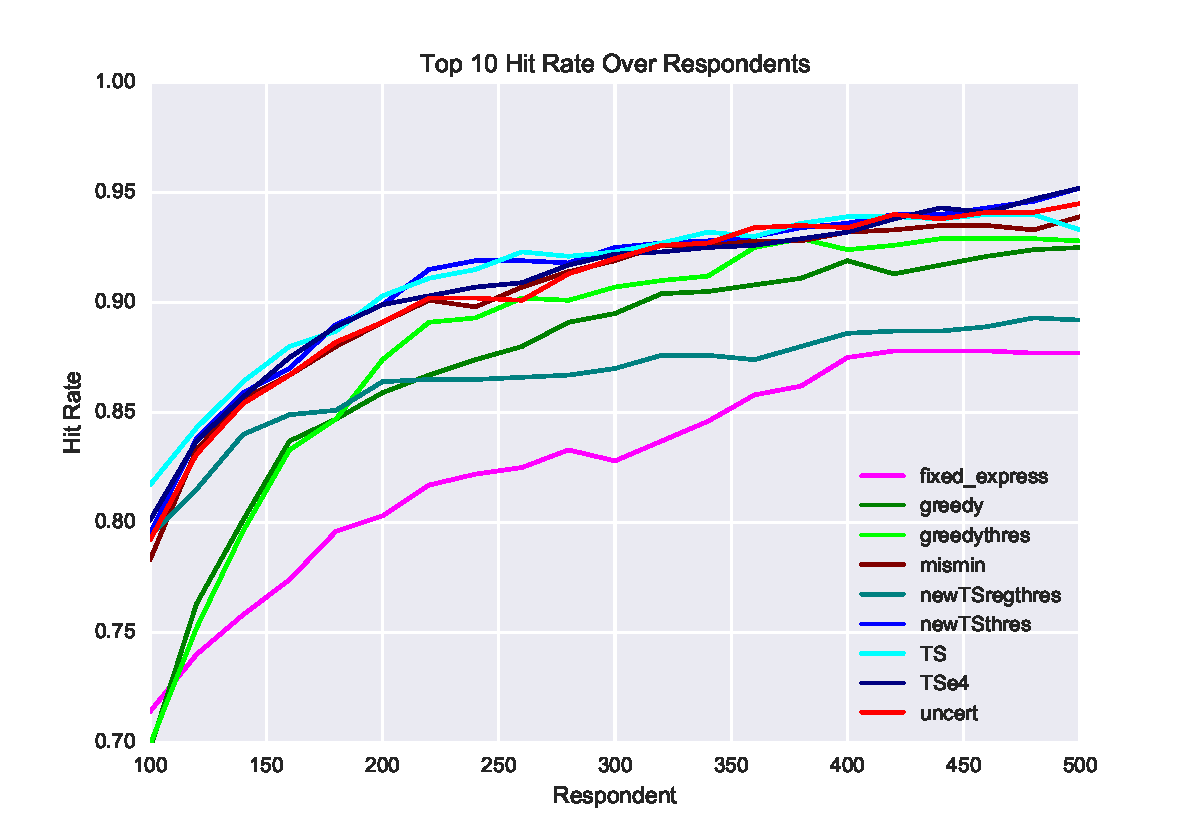
\includegraphics[width=.8\textwidth]{plots/hr120v20k10.pdf} }}%
	\end{center}
\end{figure}

%\eric{Please make y-axes the same across all k for the K120 L20 problem.}


\begin{figure}%
    \caption{Hit Rates for Top $k=\{20,40\}$ with 120 items.}%
    \label{fig:K120_L20_k20hit_k40hit}%
 	\begin{center}
    \subfloat[Top 20]{{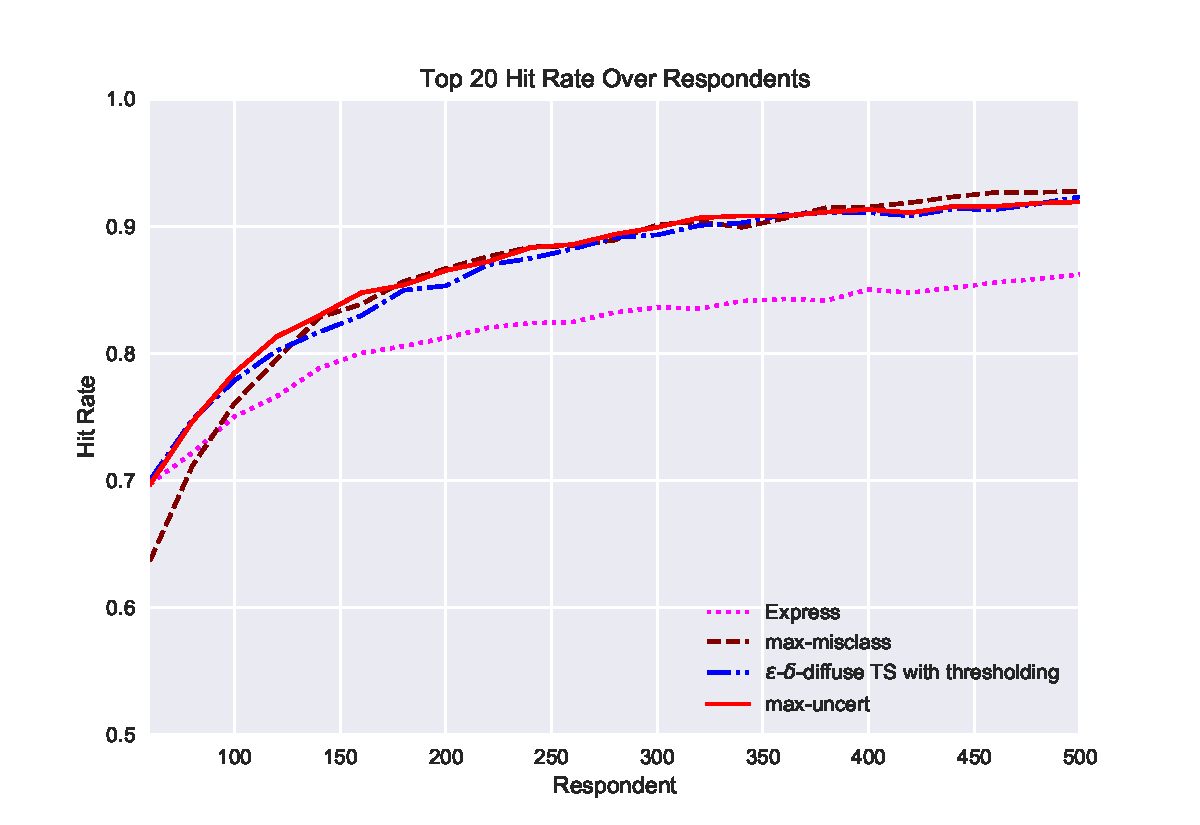
\includegraphics[width=.8\textwidth]{plots/hr120v20k20.pdf} }}%
    \qquad
    \subfloat[Top 40]{{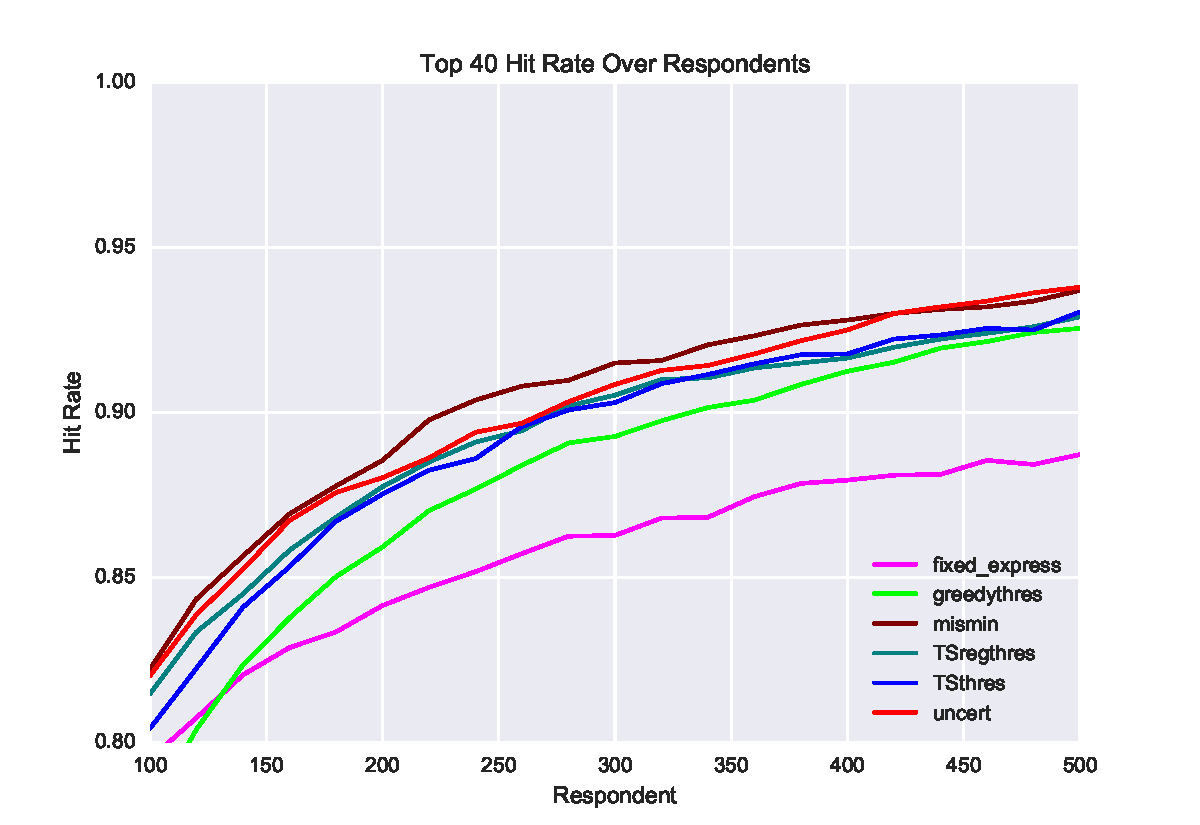
\includegraphics[width=.8\textwidth]{plots/hr120v20k40.pdf} }}%
    \end{center}
\end{figure}

%\eric{Please make y-axes the same across all k for the K120 L20 problem.}

% \begin{figure}
% \caption{3 Hit Rate with 120 items}
% 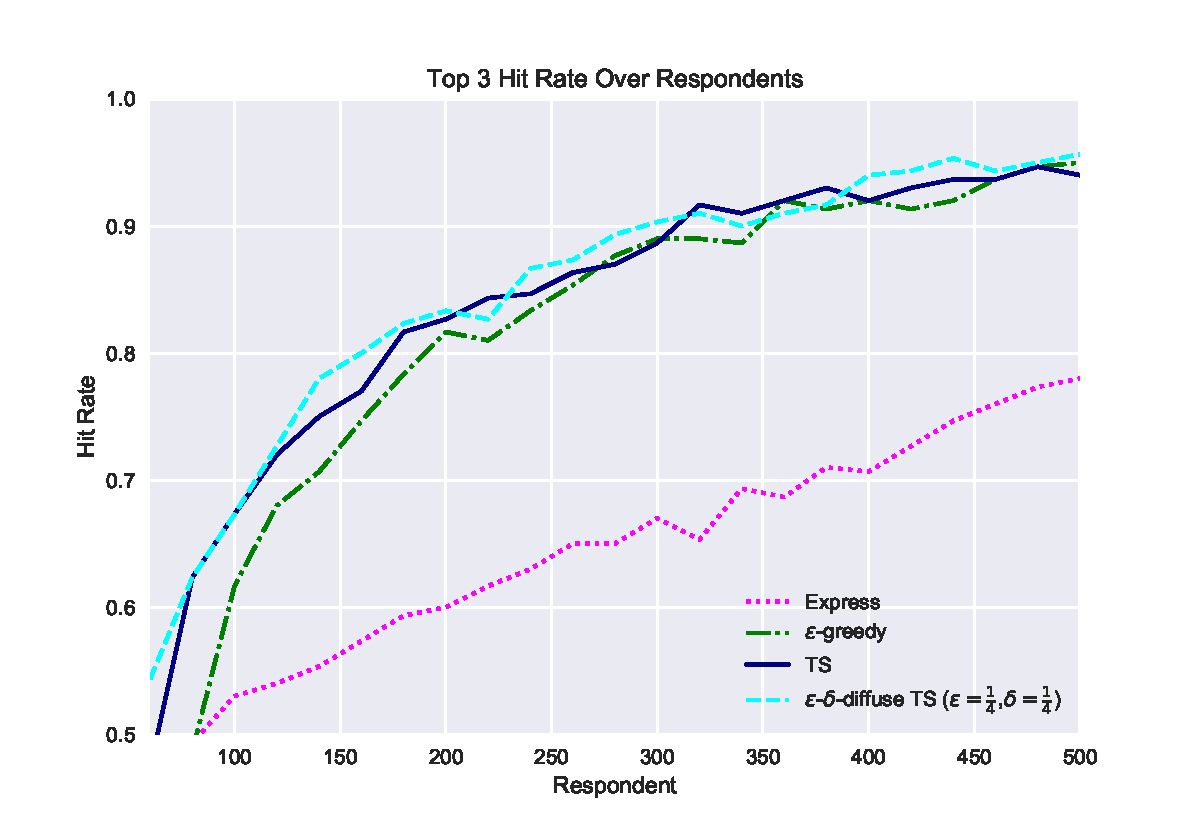
\includegraphics[width=1\textwidth]{plots/hr120v20k3.pdf}
% \label{fig:3hit}
% \end{figure}
% \begin{figure}
% \caption{10 Hit Rate with 120 items}
% 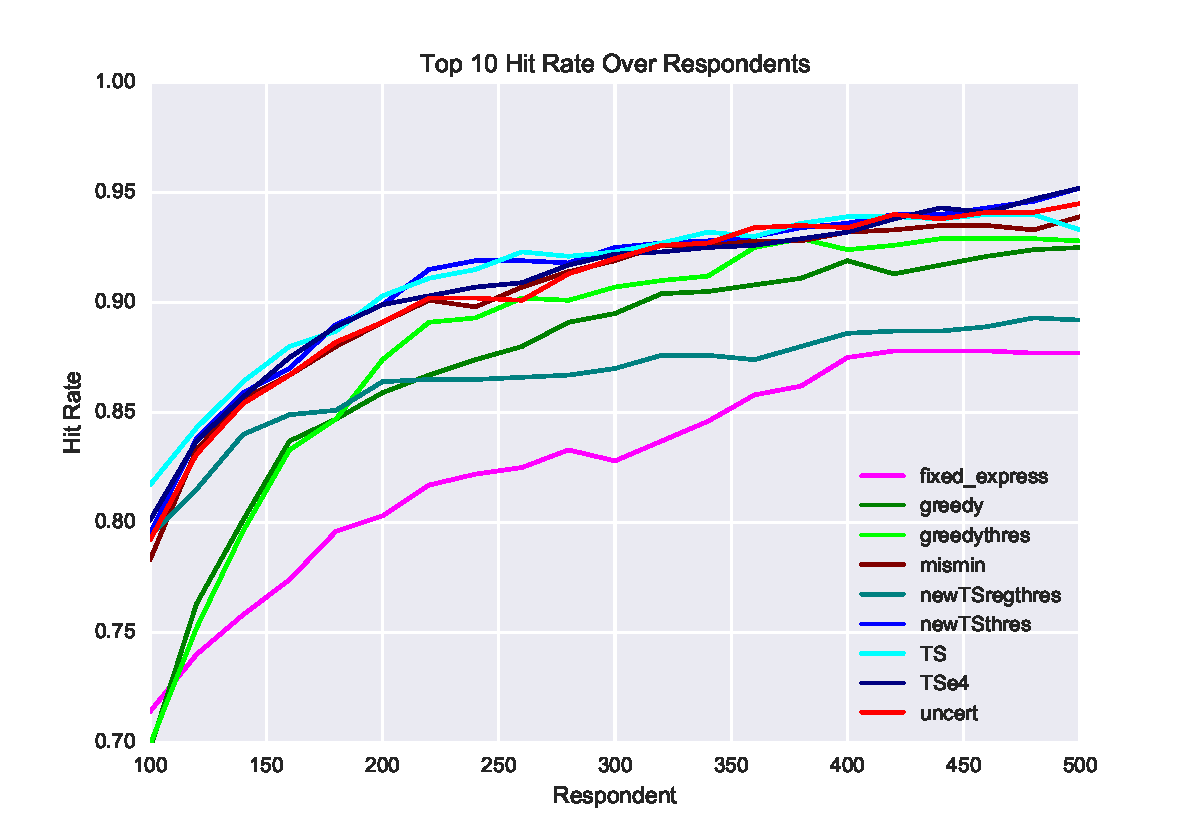
\includegraphics[width=1\textwidth]{plots/hr120v20k10.pdf}
% \label{fig:10hit}
% \end{figure}

% \begin{figure}
% \caption{20 Hit Rate with 120 items}
% 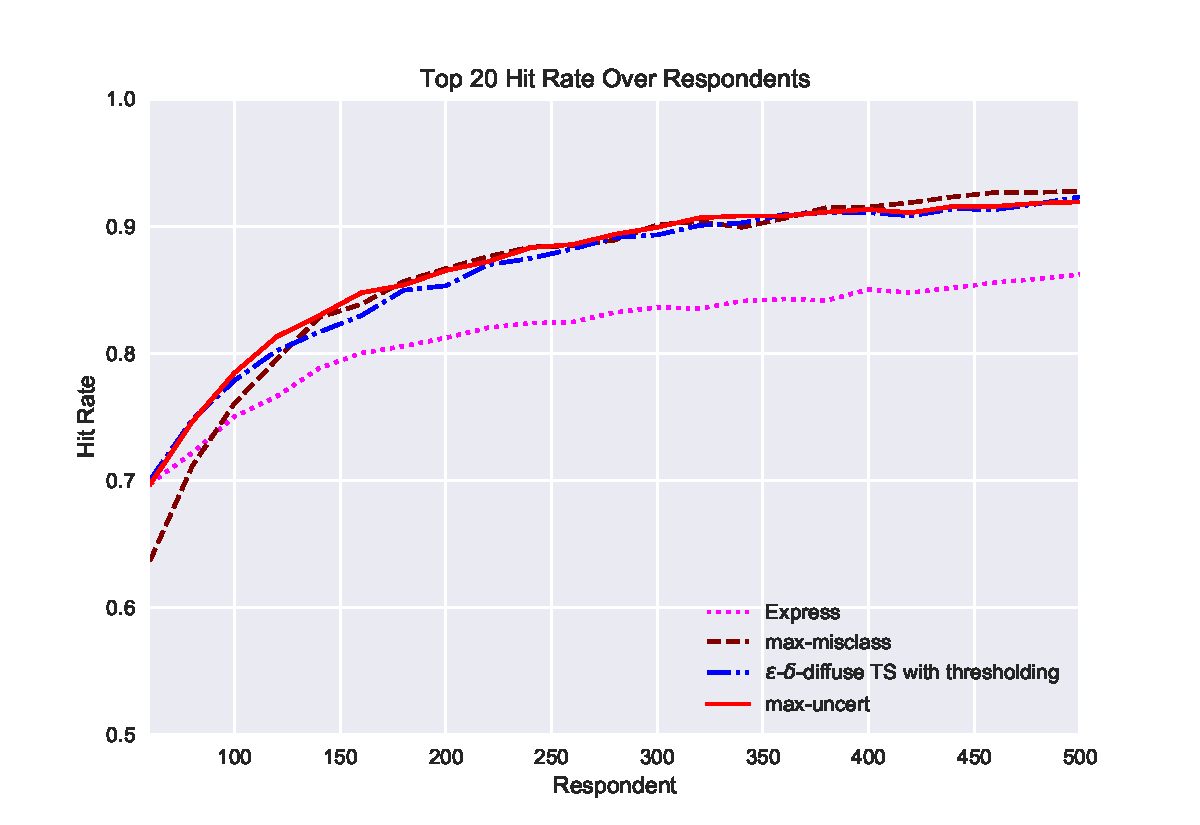
\includegraphics[width=1\textwidth]{plots/hr120v20k20.pdf}
% \label{fig:20hit}
% \end{figure}
% \begin{figure}
% \caption{40 Hit Rate with 120 items}
% 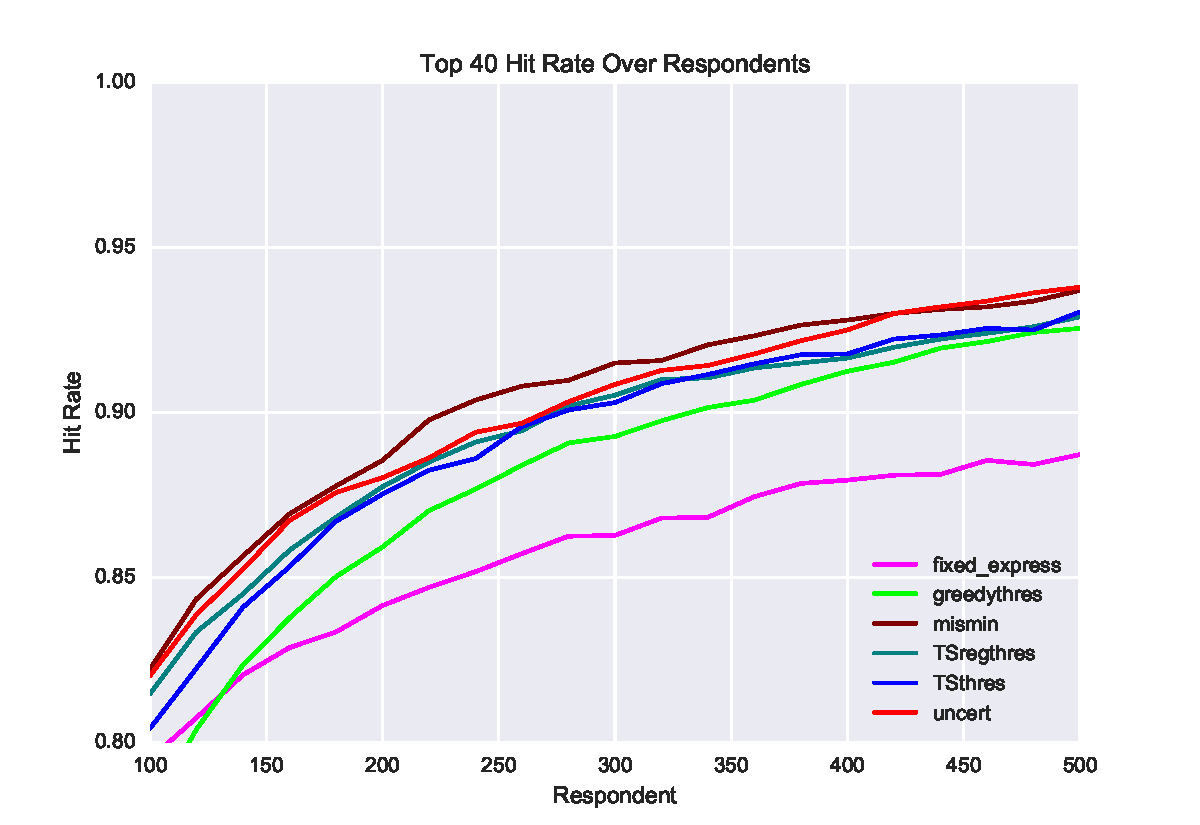
\includegraphics[width=1\textwidth]{plots/hr120v20k40.pdf}
% \label{fig:40hit}
% \end{figure}




\begin{table}
\caption{Top k Hit Rate for Various Algorithms after the 260th and 500th Respondent with 120 Items }
\label{table:at_260_500}
\begin{center}
\begin{tabular}{llllllllll}
\hline 
\hline
\multicolumn{10}{l}{(a) After 260 respondents}\\
k &  \fixedexpressS&\egreedyS&\egreedythresS&\tsS&\edtsS&\tsthresS&\edtsthresS& \misminS& \uncertS \\ \hline
  3 & 0.65 &   0.85 &  0.86 &   0.86 & 0.87 & 0.78 & 0.86 &    0.88 &   0.84 \\
  10 &  0.83 &   0.88 & 0.90 &   0.92 & 0.91 & 0.87 & 0.92 &    0.91 &   0.90 \\
  20 & 0.82 & 0.78 &  0.86 & 0.83 & 0.82 & 0.86 & 0.88 &  0.88 &   0.89 \\  
  40 &  0.86 &   NA &  0.88 &  NA & NA & 0.89 & 0.90 &  0.91 &   0.90 \\
\hline
\hline
\end{tabular}
\begin{tabular}{llllllllll}
\multicolumn{10}{l}{(b) After 500 respondents}\\
k &  \fixedexpressS&\egreedyS&\egreedythresS&\tsS&\edtsS&\tsthresS&\edtsthresS& \misminS& \uncertS  \\
\hline
   3 & 0.78 &   0.95 & 0.93 & 0.94 & 0.96 & 0.83 & 0.97 &    0.95 &   0.94 \\
  10 &  0.88 &   0.93 &  0.93 &   0.93 & 0.95 & 0.89 & 0.95 &    0.94 &   0.95 \\  
  20 &  0.86 &   0.83 & 0.91 &  0.86 & 0.87 & 0.89 & 0.92 &  0.93 &   0.92 \\ 
  40 &  0.89 &   NA & 0.93 & NA & NA & 0.92 &  0.94 & 0.94 & 0.94 \\
\hline 
\hline
\end{tabular}
\end{center}
\end{table}




% \begin{table}
% \caption{Top k Hit Rate for Various Algorithms at the 260th Respondent with 120 Items}
% \label{table:at260}
% \begin{center}
% \begin{tabular}{llllllllll}
% \hline   k &  fixed\_express &  greedy &  greedythres &  mismin &    TS &  TSe4 &  TSregthres &  TSthres &  uncert \\ \hline  3 &          0.650 &   0.853 &        0.860 &   0.883 & 0.863 & 0.873 &       0.850 &    0.893 &   0.840 \\  10 &          0.825 &   0.880 &        0.902 &   0.907 & 0.923 & 0.909 &       0.909 &    0.907 &   0.901 \\  20 &          0.824 &   0.784 &        0.863 &   0.885 & 0.825 & 0.820 &       0.869 &    0.879 &   0.886 \\  40 &          0.857 &   NA &        0.884 &   0.908 & NA & NA &       0.895 &    0.888 &   0.897\end{tabular}
% \end{center}
% \end{table}

% \begin{table}
% \caption{Top k Hit Rate for Various Algorithms at the 500th Respondent with 120 Items}
% \label{table:at500}
% \begin{center}
% \begin{tabular}{llllllllll}
% \hline   k &  fixed\_express &  greedy &  greedythres &  mismin &    TS &  TSe4 &  TSregthres &  TSthres &  uncert \\ \hline   3 &          0.780 &   0.950 &        0.933 &   0.950 & 0.940 & 0.957 &       0.917 &    0.947 &   0.943 \\  10 &          0.877 &   0.925 &        0.928 &   0.939 & 0.933 & 0.952 &       0.940 &    0.947 &   0.945 \\  20 &          0.862 &   0.827 &        0.914 &   0.928 & 0.863 & 0.868 &       0.916 &    0.914 &   0.919 \\  40 &          0.887 &   NA &        0.926 &   0.937 & NA & NA &       0.929 &    0.927 &   0.938 \end{tabular}
% \end{center}
% \end{table}


We find performance depends on the hit rate measure relative to the number of items selected ($k$ vs $L$).
For $k \ge L$ the better performers are Greatest Uncertainty with random perturbations (\uncert) and Misclassification Minimization with random perturbations (\mismin). Indeed these two methods also perform nearly as well as the other winners in the $k < L$ condition. But the $\epsilon$-diffuse Thompson sampling with thresholding (\edtsthres) and without thresholding (\edts) perform best when $k<L$. 

But the differences among the other algorithms are also telling. We find that Thompson Sampling (\ts) alone has its limits. It is constructed to select the best items (and eventually, only the best item), so it can do quite well if we only care about identifying a small number of items (the cases $k=3,10$). But is not suited for the active learning problem generally, especially when being evaluated on identifying a larger top set, for instance, when we care about the hit rate for all items in the survey (the case $k=L=20$). While the \edts adds exploration to improve its performance for the other cases, that extra exploration does not direct resources toward the places that matter most in this active learning problem: the areas of high uncertainty at the decision boundary, not just near the top of the list and not scattered randomly.  

\begin{figure}%
    \caption{Frequency of item shown for \edts and \edtsthres}%
    \label{fig:Frequency}%
 	\begin{center}
    \subfloat[]{{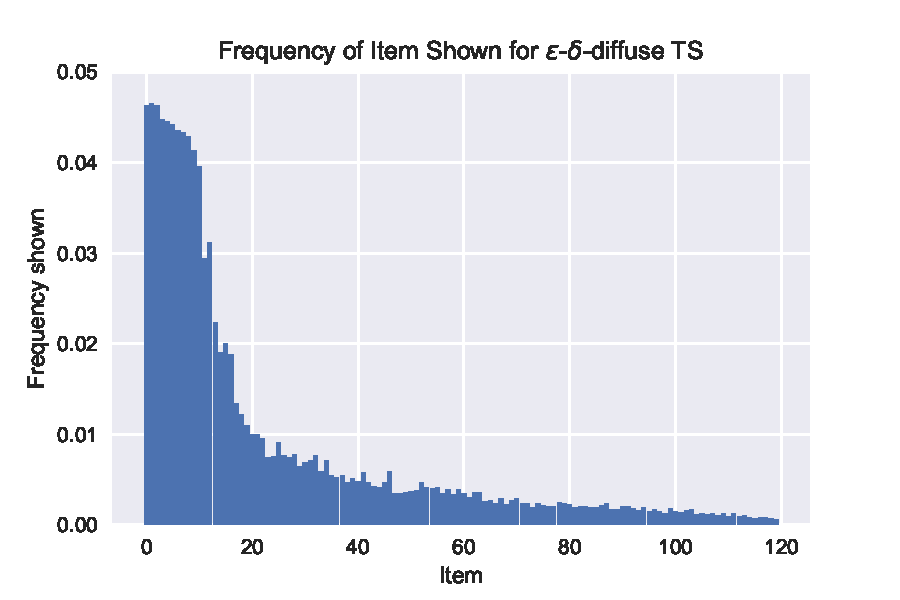
\includegraphics[width=.8\textwidth]{plots/edTSfreq.pdf} }}%
    \qquad
    \subfloat[]{{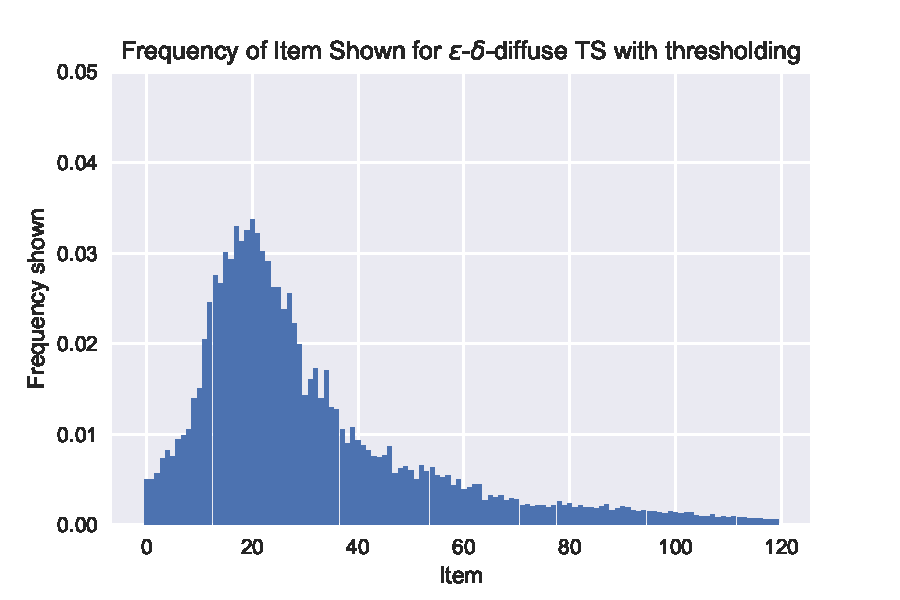
\includegraphics[width=.8\textwidth]{plots/edTSthresfreq.pdf} }}%
	\end{center}
\end{figure}

Therefore, why do the threshold-based policies, \edtsthres, \uncert and \mismin, outperform those without thresholds? Take a simple example of showing 3 items to a respondent out of 6 items, called A,B,C,D,E, and F, where we want to identify the top 3 items. Let A,B,C,D,E,and F be the utility order. Say at some point we are certain that A and B are in the top 3 and E and F are not. An algorithm without thresholding would pick A,B and either C or D. A will be chosen as the best and C or D will be chosen as the worst, giving us no new information. An algorithm with thresholding will pick C and D and either B or E. Either way the respondent will give a comparison of C and D which gives information as to which one is in the top 3. This is illustrated in Figure \ref{fig:Frequency} where you can see that \edts really focuses on the top items and \edtsthres gives more of a spread but a focus on items that are near the rank 20 item.

%\eric{Add plots highlighting these differences under a few conditions} 

% \eric{Add a Takeaway from each section beginning here.} In conclusion, \textbf{we find ... }


\section{Robustness tests} \label{sec:robust}

\subsection{Misinformed Starts (When Early Responders Are Horribly Non-Representative)}

%\alexander{Look at hr120v20k3moremis1top10.pdf, hr120v20k3moremis2top10.pdf, hr120v20k3moremis2top5.pdf, hr120v20k3moremis1top5.pdf, and see if you want to add in those results (for the 1st 150 respondents percentile of top 3 items is (resp number)/2)}

What would happen if the first 50 respondents we interviewed were actually not very representative of the average preferences for the sample?  What if we tried to throw Adaptive MaxDiff off the scent?  In fact, let's consider a worst-case scenario: the first responders actually believe \textit{nearly the opposite} from the rest of the sample.\\
For the simulations reported in table \ref{table:120mis}, the first 50 robotic respondents mimicked randomly drawn human vectors of utilities as before but were diabolically manipulated to behave as if the top 3 true items were actually nearly the worst in preference (we set the utilities for the top 3 true items for the population equal to the bottom 25th percentile utility item for each respondent).  After this misinformed start, the remaining respondents represented well-behaved respondents drawn using bootstrap sampling as before, with true individual-level preferences as given in the original dataset donated by Procter \& Gamble.\\

\begin{table}
\begin{tabular}{llllllllll}
\hline   Resp &  \fixedexpressS&\egreedyS&\egreedythresS&\tsS&\edtsS&\tsthresS&\edtsthresS& \misminS& \uncertS   \\ \hline    260 &   0.09 &   0.30 & 0.24 & 0.07  & 0.35 & 0.07 &  0.36 & 0.25 &   0.27 \\
  500 &  0.25 &   0.57 &  0.49 &  0.13 & 0.54 &   0.1 &    0.64 & 0.54 &  0.50  \end{tabular}
\begin{center}
\caption{Top 3 Hit Rate for Various Algorithms at the 260th and 500th Respondent for the 120 item data set with Misinformed Start}
\label{table:120mis}
\end{center}
\end{table}

Our diabolical simulation of a misinformed start is worse than anything you would realistically see in practice, so it is a strong test of the robustness of the Adaptive MaxDiff approach. This suggests robustness to non-stationarity in preference or self-selection of respondents during the sampling window. We created 50 misinforming early responders because in practice we are never guaranteed that the first responders represent a fair and representative draw from the population.  In fact, depending on how rapidly we invite a panel of respondents to take the survey, the first 50 respondents may share some atypical characteristics (e.g. anxious and available to take the survey at your launch time).  It would be a bad thing if our adaptive approaches performed well in simulations with well-behaved respondents, but fell apart under more realistic conditions. \\

We illustrate the robustness in Table \ref{table:120mis}. One critical point to note is that the standard Bandit MaxDiff TS approaches preform worst than Fixed Express MaxDiff under Misinformed Starts.  The extra randomness Bandit MaxDiff $\epsilon$-diffuse TS approach as well as in the other methods  is essential in allowing them to continue investigating the value of some lesser chosen items with enough frequency among later respondents, even if the prior respondents seem to have generally rejected them.

\subsection{Effect of increasing number of items}
\begin{table}
\begin{center}
\begin{tabular}{lllllllllll}
\hline   k &  \fixedexpressS & \egreedyS&\egreedythresS&\tsS&\edtsS&\tsthresS&\edtsthresS& \misminS& \uncertS \\ \hline 
3&   0.31 &   0.59 & 0.48 & 0.60 &  0.64 & 0.54 & 0.65 & 0.54 &   0.58 \\ 
10 & 0.46 &   0.61 & 0.54 & 0.63  & 0.66 & 0.58 & 0.68 & 0.68  &   0.69 \\ 
20 & 0.55 &   0.60 & 0.59 &  0.61 & 0.66 & 0.59 & 0.71 &       0.72 &   0.72\\ 
40 & 0.62 &   NA & 0.62 & NA &  NA & 0.64 & 0.70 & 0.71 & 0.72 \end{tabular}
\end{center}
\caption{Top k Hit Rate for Various Algorithms at the 260th Respondent for the 300 item data set}
\label{table:300at260}
\end{table}

\begin{table}
\begin{center}
\begin{tabular}{lllllllllll}
\hline   k &  \fixedexpressS & \egreedyS&\egreedythresS&\tsS&\edtsS&\tsthresS&\edtsthresS& \misminS& \uncertS  \\ \hline  
3 & 0.39 &  0.76 & 0.75 & 0.72 & 0.79 & 0.61 &  0.80 &  0.77 &0.78 \\
10 &  0.58 &   0.76 & 0.72 & 0.70 & 0.78 & 0.63 & 0.79 & 0.79 &   0.79\\
20 & 0.68 & 0.72 & 0.76 & 0.67 & 0.76 &  0.63 & 0.82 & 0.84 &    0.85 \\ 
40 & 0.72 &   NA & 0.75 & NA & NA & 0.69 & 0.80 &0.81 & 0.83 \end{tabular}
\end{center}
\caption{Top k Hit Rate for Various Algorithms at the 500th Respondent for the 300 item data set}
\label{table:300at500}
\end{table}
Would the benefits of Adaptive MaxDiff we observed with 120 items continue for 300 items?  While we did not have a dataset of utilities from human respondents on 300 items, we did our best to generate such a data set by leveraging the 120-item data set Procter \& Gamble shared with us.  To generate preferences across an additional set of 180 items, we randomly combined pairs of existing items according to a randomly distributed weighting scheme, with additional random variation added.  The result was a 300-item MaxDiff data set based on the original preferences of the 981 respondents.\\
The advantages seen in the 120-item results are improved upon in the results with 300 items. Tables \ref{table:300at260} and \ref{table:300at500} shows the well-informed start results. The adaptive approaches show substantial gains over the Fixed Express MaxDiff approach on the top-3,10,20,40 hit rate criterion.\\
\subsection{What about a smaller set of 40 Items?}
\begin{table}
\begin{center}
\begin{tabular}{llllllllll}
\hline   k &  \fixedexpressS & \egreedyS&\egreedythresS&\tsS&\edtsS&\tsthresS&\edtsthresS& \misminS& \uncertS  \\ \hline  3 & 0.90 & 0.97 &  0.97 &  0.97 & 0.97 & 0.97 &  0.96 & 0.94 &  0.94 \\  10 & 0.87 & 0.90 & 0.91 &  0.93 & 0.91 & 0.91 & 0.91 & 0.91 &  0.92  \end{tabular}
\end{center}
\caption{Top k Hit Rate for Various Algorithms at the 260th Respondent for the 40 item data set}
\label{table:40at260}
\end{table}

\begin{table}
\begin{center}
\begin{tabular}{llllllllll}
\hline   k &  \fixedexpressS & \egreedyS&\egreedythresS&\tsS&\edtsS&\tsthresS&\edtsthresS& \misminS& \uncertS \\ \hline    
3 & 0.93 & 0.99 & 0.99 & 0.99 & 0.99 & 0.98 & 0.98 & 0.98 &  0.99 \\  10 & 0.90 &   0.92 &  0.93  & 0.94 & 0.94 & 0.93 &    0.92 & 0.93 &  0.93 \end{tabular}
\end{center}
\caption{Top k Hit Rate for Various Algorithms at the 500th Respondent for the 40 item data set}
\label{table:40at500}
\end{table}
Our adaptive models have great advantage over fixed designs for very large numbers of items, but what happens if we have a more traditional ``large'' MaxDiff list of 40 items. Using a random 40-item subset from our original set of 120 items, we reran our simulations. \\
%By reducing the number of items to 40 and changing the number of tasks to 12, the fixed express design can now show each item an average of 1.5 times per respondent, which is much less sparse than in larger item cases.\\
By reducing the number of items to 40, the Express MaxDiff design can now show each item to every other respondent on average, which is much more than in larger item cases.
Nevertheless, our results for Adaptive MaxDiff are still better than traditional MaxDiff.

\subsection{Simulated data set}
\begin{table}
\begin{center}
\begin{tabular}{llllllllll}
\hline   k &  \fixedexpressS & \egreedyS&\egreedythresS&\tsS&\edtsS&\tsthresS&\edtsthresS& \misminS& \uncertS \\\hline  10 & 0.77 &   0.88 & 0.88  & 0.87&0.89 & 	0.88&0.89 & 0.89 &  0.88 \\  20 &  0.87 &  0.86 &   0.92  & 0.88&0.90 &  	0.93&0.94&  0.93 &  0.93 \end{tabular}
\end{center}
\caption{Top k Hit Rate for Various Algorithms at the 260th Respondent for the simulated data set}
\label{table:nice260}
\end{table}
\begin{table}
\begin{center}
\begin{tabular}{llllllllll}
\hline   k &  \fixedexpressS & \egreedyS&\egreedythresS&\tsS&\edtsS&\tsthresS&\edtsthresS& \misminS& \uncertS  \\\hline    10 & 0.85&0.92&0.92 & 0.93&0.94 & 0.92&0.94&0.93 &   0.93 \\  20 & 0.90&0.90&0.95& 0.90 &0.93 & 0.95&0.96 &0.96& 0.96 
\end{tabular}
\end{center}
\caption{Top k Hit Rate for Various Algorithms at the 500th Respondent for the simulated data set}
\label{table:nice500}
\end{table}

As a nice baseline, we sample a $\theta_i$ from a uniform distribution for $i=1,\ldots,100$. Then each respondent preference utility is sampled from a normal distribution with mean $\theta_i$ and variance 1. The rankings for each respondent are highly correlated with each other. Once again we take the top $k$ highest mean preference scores across the respondents to be the top $k$ true items. The results are in tables \ref{table:nice260} and \ref{table:nice500}.\\ The take away is that our previous results generalize to other data sets.

\subsection{Alternate data set}
\begin{table}
\caption{Top k Hit Rate for Various Algorithms after the {250th, 500th} Respondent with 86 items from the Skim group data set.
 }
\label{table:skim}
\begin{center}
\begin{tabular}{llllllllll}
\hline 
\hline
\multicolumn{10}{l}{(a) After 250 respondents}\\
k &  \fixedexpressS&\egreedyS&\egreedythresS&\tsS&\edtsS&\tsthresS&\edtsthresS& \misminS& \uncertS \\ \hline
  3 & 0.90 &   1.00 &  NA &   0.97 & 0.99 & NA & NA &    0.98 &   0.97 \\
  10 &  0.88 &   0.90 & 0.92 &   0.91 & 0.92 & 0.89 & 0.91 &    0.93 &   0.92 \\
  20 & 0.91 & 0.87 &  0.96 & 0.86 & 0.91 & 0.92 & 0.96 &  0.96 &   0.92 \\  
  40 &  0.92 &   NA &  0.95 &  NA & NA & 0.94 & 0.95 &  0.96 &   0.95 \\
\hline
\hline
\end{tabular}
\begin{tabular}{llllllllll}
\multicolumn{10}{l}{(b) After 500 respondents}\\
k &  \fixedexpressS&\egreedyS&\egreedythresS&\tsS&\edtsS&\tsthresS&\edtsthresS& \misminS& \uncertS  \\
\hline
   3 & 0.94 & 1.00 & NA & 0.98 & 1.00 & NA & NA & 1.00 &   0.99 \\
  10 &  0.91 &   0.92 &  0.93 &   0.92 & 0.93 & 0.90 & 0.93 &    0.93 &   0.94 \\  
  20 &  0.94 &   0.90 & 0.98 &  0.89 & 0.94 & 0.94 & 0.98 &  0.98 &   0.98 \\ 
  40 &  0.95 &   NA & 0.97 & NA & NA & 0.96 &  0.97 & 0.97 & 0.97 \\
\hline 
\hline
\end{tabular}
\end{center}
\end{table}
We use data from a study of claims for cleaning products from skim group. The simulation parameters are the same as the Proctor and Gamble study with the exception that we took the batch size to be 10 opposed to 20. The results can be found in table \ref{table:skim}.


\section{Alternative Performance Measure: Using True Utility as a Generalization of Hit-Rate}
\begin{table}
\begin{center}
\begin{tabular}{c | c }
$S$& Percent True Utility \\
\hline
\{1,2,3\}& 1.0 \\
\{1,2,4\}&.973 \\
\{1,2,5\}&.948 \\
\{1,3,4\}&.934 \\
\{1,3,5\}&.910 \\
\{1,4,5\}&.882 \\
\{2,3,4\}&.922 \\
\{2,3,5\}&.897 \\
\{2,4,5\}&.870 \\
\{3,4,5\}&.831 \\
\hline
\end{tabular}
\end{center}
\caption{Percent true utility for Various $S$ for Top 3 from the Procter \& Gamble data}
\label{table:PTU}
\end{table}
One might like to differentiate between an algorithm puts the top 9 items and the 11th item in the 10 top and one puts the top 9 items and the 40th item in the 10 top. A measure that differentiates the two is Percent True Utility (PTU). \\
\textbf{Exponential Weighted Utility}: For a set $S$ the exponential weighted utility is \[\mu_S=\sum_{x \in S}b(x)=\sum_{x \in S}e^{u(x)}\]
\textbf{Percent True Utility of the Top k}: The Percent True Utility (PTU) is the exponential weighted true utility of the top $k$ items that the robotic respondents identified over the maximum exponential weighted true utility that could be attained with $k$ items. Mathematically, if $\tilde{S}$ is the top $k$ items and $S$ is the current estimate of the $k$ top items then PTU is 
\[
\frac{\mu_S}{\mu_{\tilde{S}}}
\]
This can be see as a generalization of Hit-Rate. It has the advantage of differentiating as in the case the section started with though one loses the ability to easy interpret the result. In Table \ref{table:PTU} we show the PTU for various subsets of the data.
\begin{figure}
\caption{Percent True Utility of the Top 20 with 120 items}
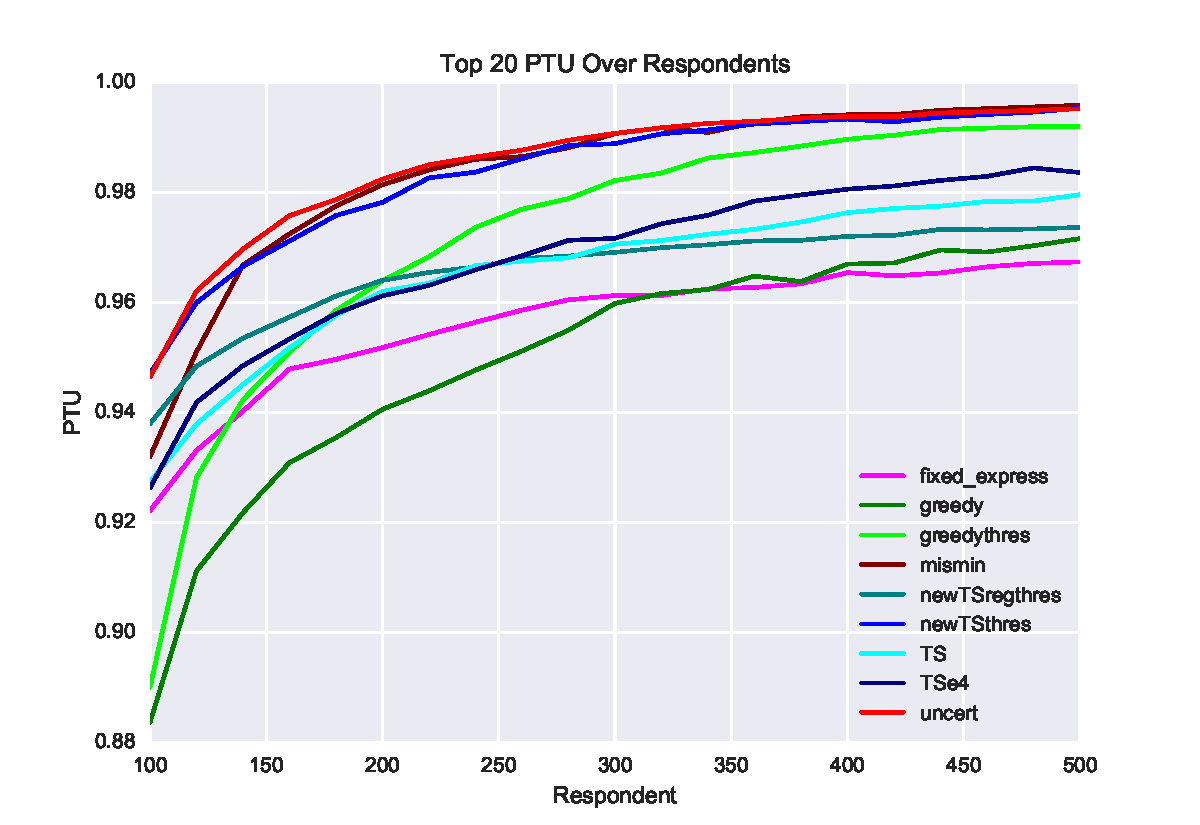
\includegraphics[width=1\textwidth]{plots/PTU120v20k20.pdf}
\label{fig:20util}
\end{figure}
Recall that for $k=20$ using the hit rate metric that Fixed Express, TS, and $\epsilon$ diffuse TS were on par with each other.
Using $k=20$ PTU, in figure \ref{fig:20util} we see that $\epsilon$ diffuse TS has a slight edge over TS which is better than Fixed Express. This means that both TS approaches put better ranked items in the top 20 then Fixed Express. In this wider consideration the methods are better than Fixed Express even though the top 20 hit rate was about the same.


\section{Stopping Rules: Posterior Distribution Regret and Value Remaining}
Almost all of the results show diminishing results as we give more surveys. Thus it becomes inefficient to keep giving surveys after a certain point. In practice we do not know this point \textit{a priori} but we would still like to know when we should stop.\\
Adapted from~\cite{scott2015multi} and~\cite{scott2010modern} for MAB, The value remaining in the experiment is the posterior distribution of $\frac{\mu_{S^*}-\mu_{S}}{\mu_{S}}$ where $\mu_{S^*}$ is the largest value of the exponential weighted utility and $\mu_{S}$ is the exponential weighted utility of the set that is most likely to be optimal, denoted $S$. This is constructed as follows, take $n$ Bayes Bootstrap draws from the posterior. Let $\mu_{S^*}^{m}$ be the max exponential weighted utility of draw $m$ and $\mu_{S}^{m}$ be the utility using the draw $m$ using the set $S$. Let $\Delta^{m}=\frac{\mu^m_{S^*}-\mu^m_{S}}{\mu^m_{S}}$.\\
\begin{table}
\begin{center}
\begin{tabular}{l | c c c c c c c c}
& \multicolumn{8}{c}{Current belief: rank order of items by utility} \\
& 1st &  2nd  &  3rd  &  4th &  5th & 6th & 7th &  8th \\
\hline
% \multicolumn{9}{l}{Posterior draws of utility} \\
Draw 1 & 4.02 &  3.50 &  5.08 & 4.16&  4.22 & 4.41 & 3.65 &  3.27 \\
Draw 2 &4.18 & 4.72 & 3.49 & 3.48 & 3.63 & 3.60 & 3.56 &  3.70 \\
Draw 3 &4.81 & 5.23 & 5.04 &  3.96 &  4.17 & 4.37 &  3.58 & 2.99 \\ 
\end{tabular}
\end{center}
\caption{Draws of the exponential utility of the items after 100 iterations}
\label{table:data}
\end{table}

\begin{figure}
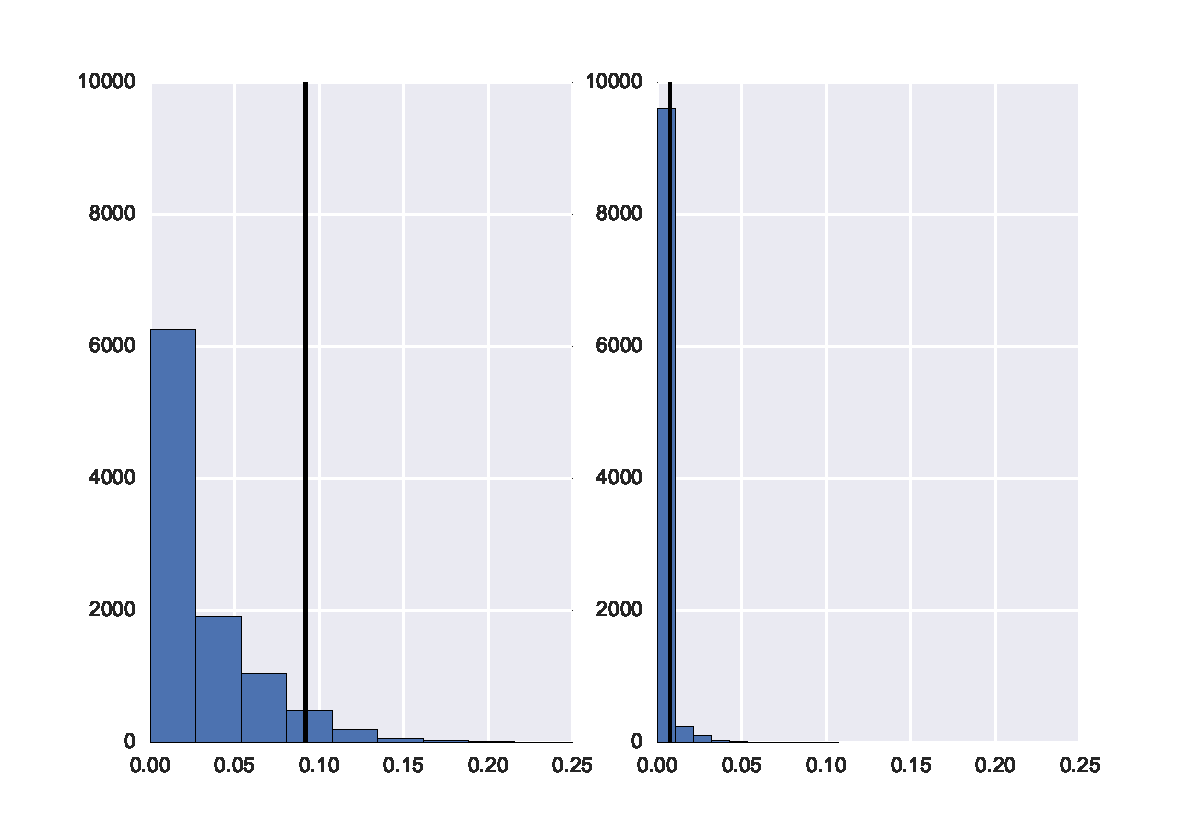
\includegraphics[width=1\linewidth]{plots/valremhist.pdf}
\caption{Two histograms of $\Delta$. Left: After 100 iterations, the potential value remaining is .092. Right: After 220 iterations, the potential value remaining is .008}
\label{fig:data}
\end{figure}
As an example see table \ref{table:data} for draws of exponential weighted utility of a single item. I put the columns in current rank order and only show the top 8 for convenience. Then $S$ is the set containing what is currently ranked as the first, second and third ranked item. Then $\mu^1_{S}=4.02+3.50+5.08=12.6$ and $\mu_{S^*}^{1}=5.08+4.41+4.16=13.65$ So $\Delta^{1}=\frac{13.65-12.6}{12.6}=.083$. Likewise $\Delta^{2}=\frac{12.6-12.39}{12.39}=.017$ and $\Delta^{3}=\frac{15.08-15.08}{15.08}=0$ (Note $\Delta^m=0$ when the $S$ contains the top utilities). The histogram of $\Delta$ after 100 iterations and 220 iterations is shown in figure \ref{fig:data}. \\
The `potential value remaining' (PVR) is the 95 quantile of the distribution $\Delta$ see figure \ref{fig:data}. After 100 iterations the PVR was 0.092. Scott's way to interpret this number is ``we do not know what the utility of $S$ is, but whatever it is, a different set might beat it by as much as 9.2\%.''\\

 %\alexander{Replace this plot with stophisted02.pdf stophistprob02.pdf and stophistTSgr02.pdf}

\begin{figure}
\caption{Average stopping time with different thresholds}
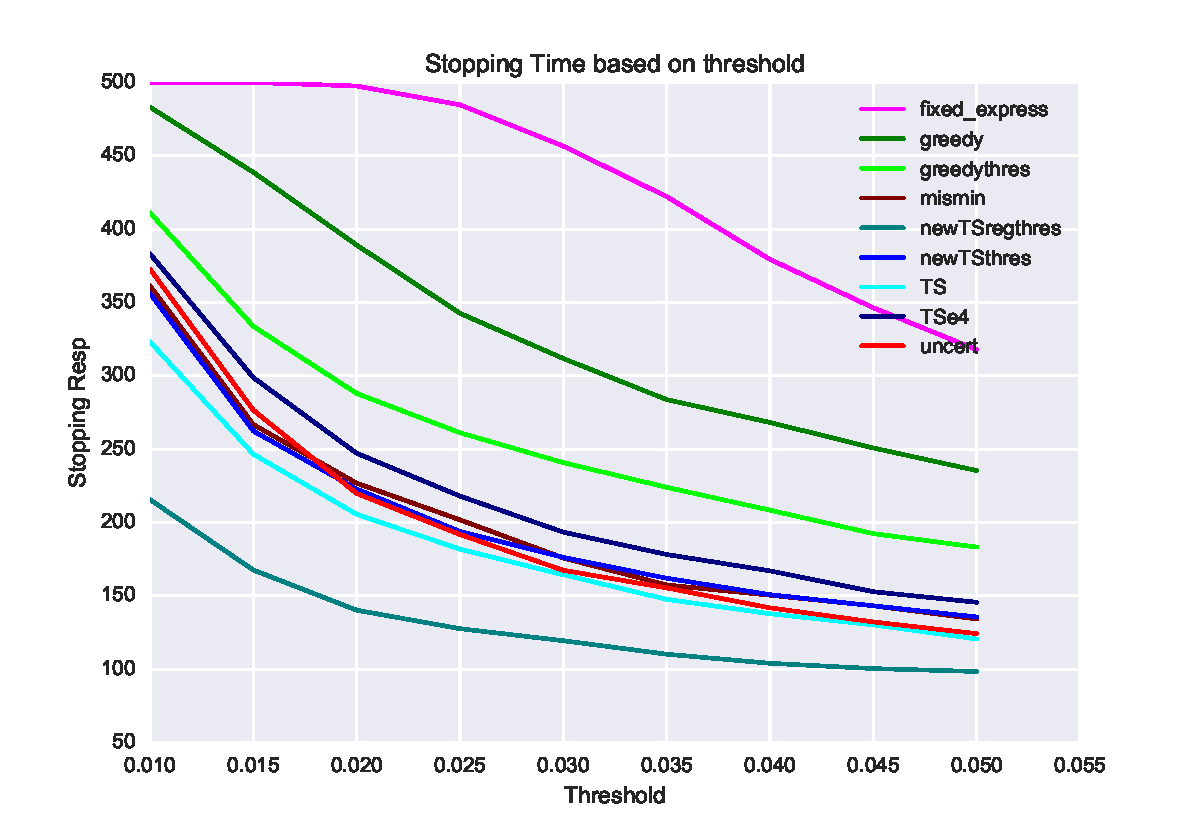
\includegraphics[width=1\textwidth]{plots/stoppingtimes.pdf}
\label{fig:st}
\end{figure}
\begin{table}
\begin{center}
\begin{tabular}{llllllllll}
\hline    &  fixed\_express &  greedy &  greedythres &  mismin &    TS &  TSe4 &  TSregthres &  TSthres &  uncert \\\hline  Avg ST  & 318 &   235 & 183 & 134 & 121 & 146 & 	98 &	136 &   124 \\  Avg hr  &  0.854 &  0.88 & 0.852&0.848 & 0.846 & 	0.866 & 0.795 &0.857 &  0.837 \end{tabular}
\end{center}
\caption{Average Stopping Time and Average Hit Rate With a threshold of .02 PVR for top 10 items}
\label{table:st2}
\end{table}
\begin{table}
\begin{center}
\begin{tabular}{llllllllll}
\hline    &  fixed\_express &  greedy &  greedythres &  mismin &    TS &  TSe4 &  TSregthres &  TSthres &  uncert \\\hline    Avg ST & 498 & 389 & 288 & 227 & 206 & 247 & 140 &223 &  220 \\ Avg hr & 0.893 &0.918&0.902& 	0.911 & 0.907& 0.912 & 0.822&0.911& 0.909\end{tabular}
\end{center}
\caption{Average Stopping Time and Average Hit Rate With a threshold of .05 PVR for top 10 items}
\label{table:st5}
\end{table}
A good stopping rule is to stop when the PVR drops below a certain threshold. See figure \ref{fig:st} for the average stopping time for different algorithms based on threshold for finding the top 10 items. Tables \ref{table:st2} and \ref{table:st5} show the average stopping time and average hit rate at those stopping time for threshold values 0.02 and 0.05. The trade-off is accuracy for how many respondents you survey. If you are using regret as a stopping rule, keep in mind that in general higher $k$ gives smaller PVR values.\\ 
%\subsection{Spearman (Rank Ordering) Correlation}
%Both hit rate and percent true utility are invariant under the ordering of the $k$ items. As a final metric we looked at the Spearmen Correlation of the true top $k$. This measures how well the algorithm's ranking of the true top $k$ items matches with the truth. For example if the 
\section{Other Sampling Schemes and Methods}
%\subsection{Changing Exploration Parameters}
%Almost all of the adaptive methods have parameters for all of these methods and the trade off is robustness against heterogeneity in the respondents verses speed of convergence. All the Greatest Uncertainty with random perturbation and Misclassification Minimization with random perturbation $c=\infty$ (or any $c \geq 250$ in the case 120 items showing 20 items to each respondent) is fixed express, and using $c=0$ , $\epsilon$-greedy with $\epsilon=1$, and $\epsilon$-diffuse TS with $\epsilon=1$ and $\delta=0$ are the same sampling scheme as fixed express. Also $\epsilon$-diffuse TS with $\epsilon=0$ is regular TS.  Our recommended ranges for the different parameters are $\frac{1}{5}\leq \epsilon \leq \frac{1}{2}$, $\frac{1}{4}\leq \delta \leq \frac{1}{2}$ and $.01 \leq c \leq 1$.
\subsection{Asking for Bests instead of Best-Worst}
Because a key assumption for using an adaptive MaxDiff approach is that the researcher is mainly interested in identifying the top few items, we wondered about the value of spending time asking respondents to identify the worst item within each MaxDiff set.  What would happen if we asked our robotic respondents only to select the best item within each set?  The results somewhat surprised us.  The value of asking respondents to indicate both best and worst within each set more than compensated for the 40\% additional effort we suppose these ``worst'' questions add to the total interview time when interviewing human respondents.
In a five item set (A,B,C,D and E) there are 10 possible 2-way comparisons. If we assume A is preferred to B and B is preferred to C and so on, then asking about only the best item will let us know A$>$B, A$>$C, A$>$D and A$>$E (4/10 comparisons).  By asking about worsts as well, for only one additional question we also add B$>$E, C$>$E, and D$>$E (7/10 comparisons), leaving only the order relationship between B, C, and D unknown.\\ 
The case of asking for bests when all respondents have same preferences that turns into the marked-bandit problem in~\cite{simchowitz2016best}. In that paper the authors give different algorithms for pulling the arms and upper and lower bounds on how many queries it takes to identify the top $k$ items with high probability. 


% \subsection{What about Double Adaptivity?}
% In~\cite{orme2006adaptive}, one of the authors presented a paper on Adaptive MaxDiff that featured within-respondent adaptation rather than what we have shown here in Bandit MaxDiff based on Thompson Sampling, which is an across-respondent adaptive approach. For the within-respondent adaptive procedure, items that a respondent indicates are worst are dropped from further consideration by that same respondent through a round-robin tournament until eventually that respondent's best item is identified.  We thought adding this additional layer of within-respondent adaptivity on top of the Bandit MaxDiff approach could additionally lift its performance.  To our surprise, this double-adaptive approach actually performed worse than Bandit MaxDiff alone in terms of hit rates for the top 3 or 10 items for the sample.  After some head-scratching (and much code checking), we determined that the lack of improvement was due to degree of heterogeneity across the robotic respondents.  For example, if we are interviewing a respondent who doesn't agree much with the overall population regarding which are the top items, it is detrimental to allow that respondent to drop from further consideration (due to judging them worst) what actually are among the globally most preferred items.  It serves the greater good for each respondent to spend increased effort judging among the items that previous respondents on average have judged as potentially best.


\subsection{Drawing from the Asymptotic Distribution}
As an alternative to Bayesian bootstrapping to get draws from the posterior, one can sample from asymptotic distribution via MLE implied by the estimated mean and standard errors, sampling $u \sim N(\theta,H^{-1})$, where $\theta$ is the minimizer of the negative log-likehood and $H$ is the Hessian of the negative log-likehood evaluated at $\theta$. The sampling methods preformed about the same using draws from either Bayesian bootstrapping or the asymptotic distribution.

Finally, yet another faster allows for online updates for streaming data, without model estimation. A benefit of MaxDiff tasks is the number of pairwise comparison is implies with one best-worst pair. One, albeit limited way to use this information, would be to act as if the respondent actually did state all of those comparisons. Then for each pair, we can assign a 'win' the more preferred item and a 'loss' to the others. By merely tallying the number of wins out of comparisons for each item, we have its own 'win percentage' in its contests against other items that it has faced so far. This is a noisy measure of proxy for its underlying utility. Appreciating this is an average as $\hat{p}_{win}$, we can describe its standard error, $se_{win}$, to be used for Thompson Sampling as follows:
\begin{align}
\hat{p}_{k,win} &= n_{k,wins} / n_{trials} \\
\text{se}_{k,win} &= \sqrt{  \frac{ \hat{p}_{k,win} (1-\hat{p}_{k,win}) } {n_{trials}}  } \\
\end{align}

The mean and variance can be used for sampling from the distribution of `winning percentages'. This can be done using \ts or \edts. For \ts, for example, after sampling one $p_{k,win}^{ts}$ for each of the $k=1,\ldots,K$ items independently, then simply rank order and identify the top set of those values. For \edts, do this for two different Normal distributions, one with $\text{se}_{k,win}$ and one with inflated standard error, $\delta \text{se}_{k,win}$.

%\subsection{Other Sampling Schemes}
%TO DO: change this section
%In ~\cite{russo2016simple}, the author analyses different Bayesian algorithms for identifying the best arm. One point he makes is that Thompson Sampling is not effective for purely exploration problems. TS leads to oversampling the top item and not getting good enough estimates the second best items to conclude with high enough confidence that the top item is the top item. He gives a variation Top-Two Thompson Sampling which is better for the best-arm identification problem. This is choosing the best arm with probability $\beta$ and choosing the second best arm with probability $1-\beta$. One way to implement this in MaxDiff surveys is top pick the top 30 items and for each item with rank $i$ with probability $1-\beta$ replace that item with the rank $i+30$ ranked item.\\
%While our problem is purely exploration, the nature of MaxDiff survey causes us to show $L$ items to every respondent, putting a limit on how much we are sampling the each item. As a result when $k$ is less $L$ we do not run in to the same estimation problems as in MAB problem. Though as we saw in PVR, adding randomness can improve the speed of parameter estimates in the same spirit as Russo's paper.\\

%\subsection{Thompson Sampling for purely exploration problems}

%\begin{figure}
%\caption{30 Hit Rate with 120 items}
%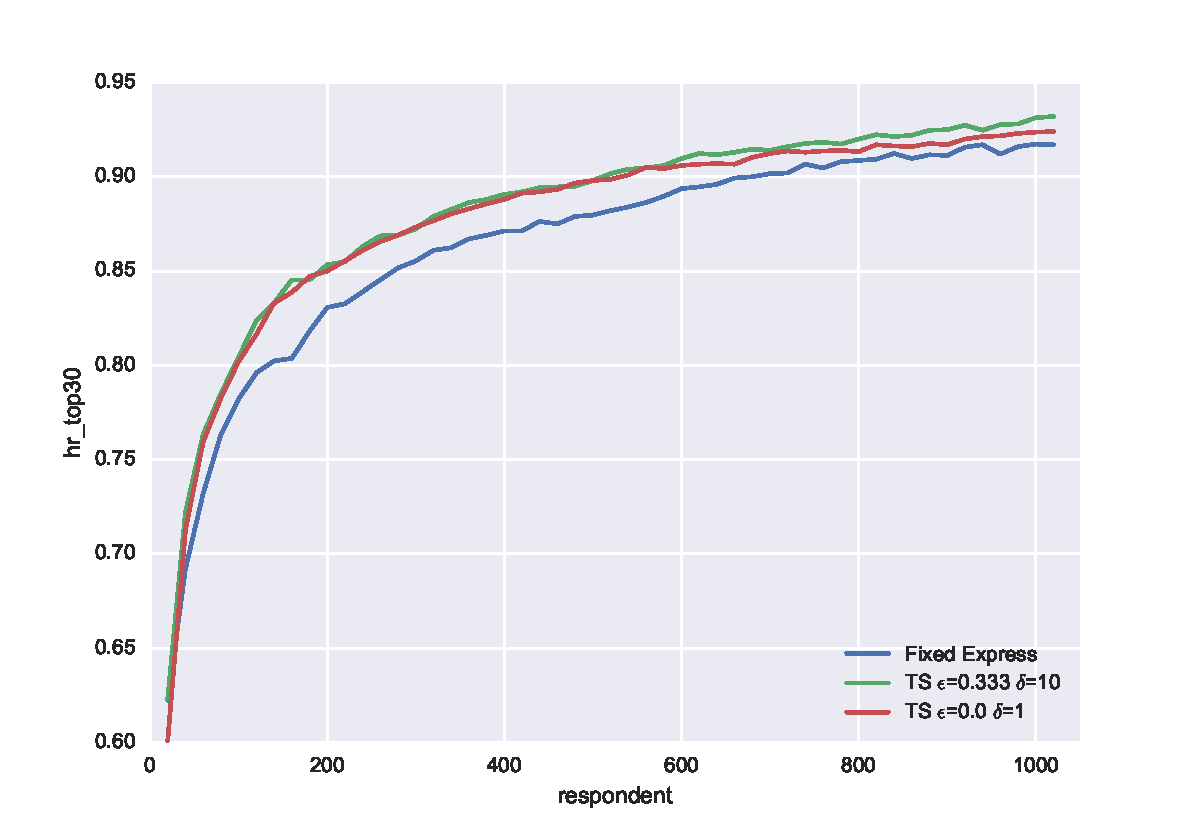
\includegraphics[width=1\textwidth]{plots/30hitrate120show3.pdf}
%\label{fig:30hit}
%\end{figure}
%Consider \ref{fig:30hit}, while MAB methods still gives a edge over fixed sparse the gains are much less. One reason is that TS sampling will  
%at is considered in ~\cite{toubia2007adaptive}, but for a different type of survey. Instead of showing a series of items and ask respondents to pick the best and worst from a list, the survey shows the respondents one item and asked to rate it using the binary choice good or bad. With each query they get information on one item. As a result the authors show fewer items to each respondent. Similar to our approach, the authors devise adaptive approaches that use previous ratings to decide the what items to show the next respondent.  Unlike our approach, they sample items more that are likely to be misclassified by looking at items close to the threshold between top items and bottom items (not top items).\\
%It is interesting to note that their best preforming solution is similar in spirit to our method of $\epsilon$-Diffuse TS. In implementation their method uses a beta distribution and can calculate their score directly instead of taking a sample. They then add noise from a normal distribution to each of the scores and show the top scoring items to the next respondent. Despite the differences, the similarity between their best method and is $\epsilon$-Diffuse TS striking.


\subsection{What about Sparse MaxDiff vs. Express MaxDiff?}
In ~\cite{wirth2012largeset}, the authors compared non-adaptive Sparse MaxDiff and Express MaxDiff at the Sawtooth Software Conference.\\
\textbf{Fixed Sparse MaxDiff}: we showed each item to each respondent an equal number of times (if possible).  With 120 items, 12 sets, and 5 items per set each item appeared on average $\frac{12*5}{120} = 0.5$ times per respondent. \\
 We compared the results using our simulation and found a modest edge in performance for Express MaxDiff (Sparse ending at 85.6\% for top 10 hit rate and Express ending at 87.7\%).

\section{Conclusions and Future Research}

Beyond the particular idea screening problem, our problem setting, identifying the top set of items with choice data collection, serves as an illustration of a broader framework. More broadly, we align the choice data collection process with managerial objectives. By aligning the two, we can improve efficiency and scalability for big data collection via choice experiments. We find we can ``get more for less,'' by improving precision only where it matters for decision making, using a smaller sample size compared to existing methods. While our work can generalize, we demonstrate its viability empirically with MaxDiff, as it is an increasingly popular and important choice experiment method. 

We also contribute ideas to the literature and practice. We frame choice task data collection as best arm identification multi-armed bandit problem and active learning problem. During the process of data collection, we adaptively yet strategically learn preferences in order to maximizing our accuracy of identifying the best set of items. The faster we begin identifying those best items, the more we include them in questions, improving the precision of estimates. Most importantly for practice, we can identify those items faster, stopping data collection sooner, saving money in the form of number of respondents and time. 


Our results suggest that if your main purpose in using large item lists in MaxDiff is to identify the top items for the population (not individual-level estimates), then adaptive MaxDiff approaches can be 3x more efficient than standard Express MaxDiff designs.  You are potentially wasting 66 cents of each dollar spent on data collection by not using adaptive MaxDiff.\\
Adaptive MaxDiff leverages information from prior respondents to show more effective trade-offs to later respondents (tending to oversample the stars). Greatest Uncertainty with random perturbations, Misclassification Minimization with random perturbations, $\epsilon$-diffuse Thompson sampling with thresholding, and $\epsilon$-greedy with thresholding under any choice of $k$. Additionally $\epsilon$-diffuse Thompson Sampling works well when $k<L$ and $\epsilon$-greedy works well when $k<<L$. One author prefers Misclassification Minimization with random perturbations and $\epsilon$-diffuse Thompson sampling with thresholding in all cases.\\
Even in the face of diabolically imposed misinformed starts (horribly unrepresentative first responders), these adaptive MaxDiff approaches are robust and self-correcting.\\
Although our simulations involve 120-item and 300-item tests, we expect that even greater efficiency gains (compared to standard Express MaxDiff designs) may occur with 500-item (or more) MaxDiff studies. For studies using 40 respondents, our simulation showed a 2x advantage in efficiency over fixed MaxDiff designs. Though not as dramatic, this is still a sizable boost.\\
Future research should test our findings using human respondents.  Using an adaptive process that focuses on comparing best items may result in a more cognitively difficult task than a standard level-balanced, near-orthogonal approach.  The greater expected within-set utility balance may lead to higher response error which may counteract some of the benefits of the adaptive approaches.  However, based on previous research~\cite{orme2006adaptive} that employed within-respondent adaptivity, the additional degree of difficulty that the Bandit adaptive approach could impose upon individual respondents (owing to utility balance) would probably not counteract the lion share of the benefits we've demonstrated using simulated respondents.\\
This paper also introduces a framework that links conjoint methods and multi-armed bandit methods. Much like adaptive conjoint methods began with aggregate adaptation and then progressed to individual-level adaptive, so we propose an aggregate adaptive approach. But future could explore methods using fully heterogeneous models, and adapting within each individual. A partially pooled model will be useful here, as it is with other adaptive conjoint methods. \\
Our method relates to existing adaptive conjoint just as M-efficiency criterion is to D-efficiency.  Unlike M-efficiency designs where the researcher decides the managerial weight of different factors a priori, we know which of the items should receive more weight. Instead, that is exactly what we want to learn actively. \\
We should note that as of this article's publication date, Sawtooth Software does not offer Adaptive MaxDiff as a commercial tool, but it is currently testing versions of it to be commercially available MaxDiff software. 








% Acknowledgments here
\ACKNOWLEDGMENT{%
% Enter the text of acknowledgments here
}% Leave this (end of acknowledgment)


% Appendix here
% Options are (1) APPENDIX (with or without general title) or 
%             (2) APPENDICES (if it has more than one unrelated sections)
% Outcomment the appropriate case if necessary
%
% \begin{APPENDIX}{<Title of the Appendix>}
% \end{APPENDIX}
%
%   or 
%
% \begin{APPENDICES}
% \section{<Title of Section A>}
% \section{<Title of Section B>}
% etc
% \end{APPENDICES}

% References here (outcomment the appropriate case) 

% CASE 1: BiBTeX used to constantly update the references 
%   (while the paper is being written).
\bibliographystyle{informs2014} % outcomment this and next line in Case 1
\bibliography{source} % if more than one, comma separated

% CASE 2: BiBTeX used to generate mypaper.bbl (to be further fine tuned)
%\input{mypaper.bbl} % outcomment this line in Case 2

\end{document}


